%% =====================================================================
%% Perturbaciones proactivas para impedir el entrenamiento no autorizado de
%% modelos de visión por computador: revisión sistemática de la literatura.
%% =====================================================================
\documentclass[pdflatex,sn-mathphys-num]{sn-jnl}

\usepackage[utf8]{inputenc}
\usepackage[T1]{fontenc}
\usepackage[spanish,es-noshorthands,es-tabla]{babel}
\usepackage{graphicx}
\usepackage{multirow}
\usepackage{amsmath,amssymb,amsfonts}
\usepackage{amsthm}
\usepackage{mathrsfs}
\usepackage[title]{appendix}
\usepackage{xcolor}
\usepackage{textcomp}
\usepackage{manyfoot}
\usepackage{booktabs}
\usepackage{array}
\usepackage{longtable}
\usepackage{tabularx}
\usepackage{tikz}
\usetikzlibrary{arrows.meta,positioning,calc}

%% Encabezados fijos de la clase, traducidos
\AtBeginDocument{%
  \renewcommand\refname{Referencias}%
  \renewcommand\tablename{Tabla}%
  \renewcommand\figurename{Figura}%
  \renewcommand\appendixname{Apéndice}%
  \renewcommand\abstractname{Resumen}%
  \def\keywordname{Palabras clave}%
}

%% Columnas de párrafo: X ponderadas para tablas a todo el ancho
\newcolumntype{Y}[1]{>{\hsize=#1\hsize\raggedright\arraybackslash}X}
\newcolumntype{Z}[1]{>{\hsize=#1\hsize\centering\arraybackslash}X}
\newcolumntype{L}[1]{>{\raggedright\arraybackslash}p{#1}}
\newcolumntype{C}[1]{>{\centering\arraybackslash}p{#1}}
%% Punto de corte sin guion, para DOI y cadenas largas
\newcommand{\br}{\discretionary{}{}{}}

\theoremstyle{thmstyleone}
\newtheorem{theorem}{Teorema}
\newtheorem{proposition}[theorem]{Proposición}
\theoremstyle{thmstyletwo}
\newtheorem{example}{Ejemplo}
\newtheorem{remark}{Observación}
\theoremstyle{thmstylethree}
\newtheorem{definition}{Definición}

\raggedbottom

\begin{document}
\title[Robustez y reversibilidad de la perturbación proactiva]{Perturbaciones proactivas para impedir el entrenamiento no autorizado de modelos de visión por computador: una revisión sistemática de la literatura sobre su robustez frente a contramedidas adversarias}
\author[1]{\fnm{Glender} \sur{Vargas}}
\author[1]{\fnm{Franco} \sur{Aguilar}}
\author[1]{\fnm{Rodrigo} \sur{Calli}}
\author[1]{\fnm{Juan Jesús} \sur{Soria Quijaite}}
\affil[1]{\orgdiv{Escuela Profesional de Ingeniería de Sistemas},\orgname{Universidad Peruana Unión},\orgaddress{\city{Lima},\country{Perú}}}

\abstract{\textbf{Contexto.} Las imágenes publicadas en internet se recolectan sin autorización para entrenar clasificadores y sistemas de reconocimiento facial. Frente a ello se han propuesto perturbaciones proactivas que el titular del dato aplica a sus propias imágenes para degradar su utilidad como material de entrenamiento. La eficacia que declaran quienes las proponen difiere de la que obtienen las evaluaciones independientes. \textbf{Objetivo.} Determinar qué robustez y qué reversibilidad reportan los estudios primarios publicados entre 2020 y 2026 para estas perturbaciones frente a las contramedidas documentadas, y bajo qué modelos de amenaza se han evaluado. \textbf{Método.} Revisión sistemática conforme a PRISMA 2020 y a las guías de Kitchenham y Charters, con una ecuación de búsqueda de cuatro bloques PICO ejecutada el 14 de septiembre de 2026 en Scopus, Web of Science, IEEE Xplore y SpringerLink y una vía complementaria; selección por pares con ocho criterios de inclusión y once de exclusión, y evaluación de calidad con nueve preguntas. \textbf{Resultados.} Se identificaron 801 registros y se incluyeron 35 estudios: 22 de clasificación de imágenes, 5 de reconocimiento facial, 4 multimodales y 4 de otros dominios. Los estudios evalúan sobre todo transformaciones, aumentos de datos y entrenamiento adversarial; solo ocho evalúan una contramedida diseñada contra un mecanismo concreto. Frente al comparador sin contramedida las protecciones dejan al adversario en exactitudes bajas, pero el peor caso que declara cada proponente llega hasta el 77\,\% y, cuando un tercero diseña la contramedida con conocimiento del mecanismo, supera lo declarado por el proponente. En 17 de los 35 estudios la referencia limpia no corresponde al mismo procedimiento que la contramedida, lo que limita la comparabilidad. El análisis bibliométrico de la literatura temática muestra un crecimiento sostenido y una estructura conceptual en la que las líneas de clasificación y de reconocimiento facial ocupan regiones distintas, conectadas por términos de privacidad, ejemplos adversariales y modelos de difusión.}
\keywords{ejemplos no aprendibles, perturbación proactiva, envenenamiento de disponibilidad, entrenamiento no autorizado, reconocimiento facial, robustez, revisión sistemática}

\maketitle

\section{Introducción}\label{sec:intro}

La recolección masiva de imágenes publicadas en internet sostiene el entrenamiento de clasificadores visuales y de sistemas de reconocimiento facial sin que el titular del dato intervenga en esa decisión. Frente a este escenario ha surgido una línea de trabajo que no busca restringir el acceso al dato sino alterarlo: añadir a la imagen una perturbación imperceptible que degrade su utilidad para quien la explote sin autorización. El mecanismo original, los ejemplos no aprendibles (\emph{unlearnable examples}), introduce un ruido minimizador de error que genera un atajo estadístico correlacionado con la etiqueta, de modo que el modelo aprende el ruido en lugar del contenido y falla ante datos limpios \cite{huang2021unlearnable}. En paralelo, el linaje del ocultamiento facial persigue el mismo objetivo sobre galerías de identidades \cite{shan2020fawkes}. Ambas líneas comparten la premisa de que la protección se ejerce sobre el dato y antes de su recolección; difieren en el mecanismo de generación, en la tarea del adversario y en la etapa del sistema donde se mide el efecto.

La premisa que sostiene esta línea es empíricamente disputada. Operaciones de bajo costo, muchas de ellas ajenas a cualquier intención ofensiva, revierten buena parte de la protección declarada. Hapuarachchi y Xiong aplicaron aprendizaje por conjuntos con transformaciones no lineales sobre datos protegidos por doce enfoques distintos y obtuvieron más del 89\,\% de exactitud media, elevando el caso de One-Pixel Shortcut del 22,16\,\% al 90,38\,\% \cite{hapuarachchi2025advancing,wu2023onepixel}. Gong et al. documentan que el aumento de datos, procedimiento habitual de preprocesamiento, eleva la exactitud sobre datos protegidos por ruido minimizador de error del 21,38\,\% al 66,14\,\% \cite{gong2026armor}. Dolatabadi et al. recuperan del 7,86\,\% al 91,57\,\% en CIFAR-10 mediante purificación por difusión \cite{dolatabadi2024devil}. Existen, sin embargo, contraejemplos parciales: CUDA se mantiene en el 8,96\,\% bajo entrenamiento estándar en ImageNet-100 y resiste suavizado, aumentos y ajuste fino \cite{sadasivan2023cuda}. El cuadro resultante es el de una carrera armamentista abierta, no el de un veredicto cerrado en ninguno de los dos sentidos.

Interpretar esta divergencia exige atender a una variable que los estudios declaran de forma desigual: el modelo de amenaza. Una cifra aislada de exactitud no es interpretable sin saber qué datos protegidos entraron al entrenamiento, qué conocimiento y qué recursos tenía el recolector, y contra qué condición se comparó. Una contramedida evaluada por quien propone la protección y otra diseñada por quien conoce su mecanismo no miden lo mismo, aunque ambas se reporten como exactitud sobre el mismo conjunto de datos. La hipótesis de trabajo de esta revisión es que buena parte de la divergencia entre resultados se explica por el modelo de amenaza asumido; se examina mediante la síntesis y no se presenta como hallazgo establecido.

El término reversibilidad exige, además, una distinción que la literatura no siempre hace explícita. La recuperación del dato original por parte de un usuario autorizado, mediante una llave o un mecanismo que el titular controla, no equivale a que un recolector no autorizado elimine la protección \cite{wang2026reversible}. Las dos acepciones coexisten en el corpus y se registran por separado: esta revisión reserva \emph{reversibilidad} para la reversión por parte del adversario y \emph{reversibilidad autorizada} para la primera. De forma análoga, perturbar una consulta para evadir un reconocedor ya entrenado no demuestra protección del conjunto con el que el adversario aprende; la revisión exige evidencia de participación de los datos protegidos en el entrenamiento discriminativo.

La literatura de síntesis disponible no cubre este objeto. De las siete revisiones identificadas como relacionadas (Tabla~\ref{tab:revisiones}), dos delimitan su alcance al adversario generativo, tres son preimpresiones no arbitradas y una no cubre el constructo según su índice. La referencia más próxima, el SoK de Wenger et al., sí aborda el adversario discriminativo, pero se restringe al reconocimiento facial, es narrativo y precede a la mayor parte de la evidencia de reversibilidad publicada entre 2023 y 2026 \cite{wenger2023sok}. No se ha identificado una revisión que reúna simultáneamente tres condiciones: (i) un protocolo sistemático conforme a PRISMA 2020 y a las guías de Kitchenham y Charters, con criterios explícitos y evaluación de calidad; (ii) la cobertura conjunta de los dominios en que se ha evaluado el adversario discriminativo ---clasificación, reconocimiento facial, multimodal y otros--- bajo un mismo marco, sintetizando cómo varían la robustez y la reversibilidad entre ellos; y (iii) la persistencia frente a contramedidas como pregunta principal, explicada por el modelo de amenaza.

La segunda condición no es una preferencia de alcance. El corpus incluido reparte 22 estudios de clasificación de imágenes frente a 5 de reconocimiento facial y 4 multimodales, un desequilibrio que hace de la variación entre dominios una pregunta abierta y no un supuesto: RQ7 la plantea de forma explícita.\footnote{Un estudio recuperado por la búsqueda sostiene en su resumen que las técnicas de clase acotada desarrolladas para clasificación no son aplicables al reconocimiento facial de conjunto abierto, porque en este las identidades de entrenamiento y prueba son disjuntas y el modelo aprende geometría de \emph{embeddings} en lugar de fronteras de clase \cite{paik2026toward}. Su texto completo no se recuperó, de modo que la afirmación se registra como declarada por los autores y no como evidencia verificada.}

La pregunta principal de la revisión es: ¿qué robustez y reversibilidad reportan los estudios primarios para las estrategias y algoritmos de perturbación proactiva frente a las contramedidas adversarias documentadas en el entrenamiento no autorizado de modelos discriminativos, y bajo qué modelos de amenaza se han evaluado? El verbo que la gobierna es \emph{reportan}: la revisión sintetiza lo que la literatura mide y no realiza mediciones propias.

El resto del artículo se organiza así. La Sección~\ref{sec:antecedentes} fija las definiciones operativas y la escala de modelos de amenaza. La Sección~\ref{sec:metodo} describe el protocolo, desde la ecuación de búsqueda hasta la síntesis y el análisis bibliométrico. La Sección~\ref{sec:resultados} reporta el flujo de selección, la caracterización del corpus, la estructura bibliométrica de la literatura y la síntesis por preguntas de investigación.

\begin{table}[h]
\centering
\caption{Revisiones de síntesis identificadas como relacionadas y su alcance respecto del objeto de esta revisión.}\label{tab:revisiones}
\footnotesize
\begin{tabularx}{\textwidth}{@{}Y{0.85}Y{0.6}Y{0.85}Y{1.7}@{}}
\toprule
Revisión & Adversario & DOI o ID & Alcance respecto de esta revisión \\
\midrule
Deng et al. (2025), ACM CSUR \cite{deng2025survey} & Generativo & \texttt{\scriptsize 10.\br 1145/\br 3770916} & La taxonomía «Attacked Module» solo lista módulos generativos \\
Nguyen-Le et al. (2025), ACM CSUR \cite{nguyenle2025survey} & Generativo & \texttt{\scriptsize 10.\br 1145/\br 3771296} & Revisión del adversario generativo; no aparecen Fawkes, LowKey ni Huang et al. (2021) entre sus referencias \\
Wenger et al. (2023), IEEE S\&P \cite{wenger2023sok} & Discriminativo facial & \texttt{\scriptsize 10.\br 1109/\br SP46215.\br 2023.\br 10179445} & SoK narrativo de la línea facial, anterior a la evidencia 2023--2026 \\
Wen et al. (2026), ACM CSUR \cite{wen2026image} & Ambos & \texttt{\scriptsize 10.\br 1145/\br 3818678} & Su índice no cubre Fawkes ni ejemplos no aprendibles \\
Li et al. (2025), preimpresión \cite{li2025unlearnabledata} & Clasificación & arXiv:2503.23536 & Trata la robustez como una columna sí/no de una tabla, no como síntesis \\
Zhang et al. (2026), preimpresión \cite{zhang2026adversarial} & Ambos & arXiv:2608.04314 & Dos de sus cinco comunidades coinciden con el objeto \\
Chen et al. (2025), preimpresión \cite{chen2025survey} & Facial & arXiv:2501.08665 & Examina Fawkes, OPOM, TIP-IM, REM y ruido minimizador de error \\
\botrule
\end{tabularx}
\par\vspace{3pt}\scriptsize\raggedright No se atribuye cobertura ni ausencia de cobertura a partir del título. Las preimpresiones se registran como literatura gris de contexto y no como estudios incluidos.\par
\end{table}

\section{Antecedentes y definiciones operativas}\label{sec:antecedentes}

Una \textbf{perturbación proactiva} es una modificación del dato visual aplicada por su titular con la finalidad de dificultar su explotación no autorizada mediante entrenamiento. Se registran la norma, el presupuesto y las medidas de distorsión cuando el estudio las reporta. La ausencia de una norma explícita no constituye por sí sola un motivo de exclusión: se puntúa en la rúbrica de calidad y se documenta lo que el estudio declara. Las perturbaciones proactivas se distinguen de la desidentificación, la anonimización, la ofuscación por redes generativas, el desenfoque, las máscaras invertibles y el cifrado, que quedan fuera del alcance.

Una \textbf{contramedida} es una transformación de los datos, del procedimiento de aprendizaje o de los recursos iniciales del recolector que se evalúa para recuperar utilidad a partir de datos protegidos. Puede consistir en compresión, aumento de datos, entrenamiento adversarial, purificación, filtrado, aprendizaje por conjuntos, destilación, preentrenamiento o ajuste fino. El uso de un modelo de difusión como purificador no convierte al estudio en generativo: el criterio se aplica al modelo que el adversario finalmente entrena y a la tarea que evalúa.

El \textbf{comparador A0} es el entrenamiento con datos protegidos sin contramedida alguna. La referencia de entrenamiento con datos limpios se identifica por separado. Se denomina \textbf{protección residual} a la degradación que permanece respecto de la referencia limpia después de aplicar una contramedida, siempre bajo condiciones comparables. La exactitud recuperada respecto de A0 mide la eficacia de la contramedida y no es, por sí sola, una medida de protección residual.

El término \textbf{adversarial} designa en este trabajo una relación y no una técnica. La misma matemática opera en dos direcciones opuestas: en el ataque clásico, quien perturba la entrada es el atacante y el modelo ya entrenado falla en inferencia, de modo que el defensor es el dueño del modelo; en el escenario de esta revisión, quien perturba es el titular del dato y el modelo falla al entrenarse, de modo que el defensor es la persona. Quién ocupa el rol de adversario depende, por tanto, del modelo de amenaza declarado.

Para operacionalizar ese modelo de amenaza se adopta una escala de cuatro niveles, que se registra como la etiqueta máxima evaluada en cada estudio: \textbf{A0}, adversario ingenuo, que entrena directamente sobre los datos protegidos; \textbf{A1}, genérico, que aplica contramedidas de uso común sin conocer el mecanismo de protección; \textbf{A1.5}, preentrenado, que parte de un modelo o extractor de características entrenado con datos limpios; y \textbf{A2}, adaptativo, que conoce el mecanismo y diseña la contramedida en consecuencia. La escala no pretende ser universal ni sus niveles son dimensiones mutuamente excluyentes: un adversario puede partir de preentrenamiento y ser adaptativo a la vez. Dentro de A2 se distingue además la contramedida diseñada contra el método concreto que se evalúa (A2-e) de la diseñada contra los ejemplos no aprendibles en general o contra otra protección de la misma familia y aplicada sin adaptarla (A2-f).

\section{Metodología}\label{sec:metodo}

\subsection{Diseño del protocolo y trazabilidad}

La revisión adopta como referencia metodológica las guías de Kitchenham y Charters para revisiones sistemáticas en ingeniería de software \cite{kitchenham2007guidelines}. El reporte se organiza conforme a PRISMA 2020, con PRISMA-S para documentar las búsquedas y SEGRESS como guía complementaria del ámbito \cite{page2021prisma,rethlefsen2021prismas,kitchenham2023segress}. Estas guías orientan la transparencia del procedimiento y no sustituyen la ejecución de la selección ni la evaluación crítica.

El protocolo se congeló antes del cribado y no se depositó en un registro prospectivo externo. La trazabilidad se conserva en un registro estructurado de decisiones por registro, por etapa del flujo, y en el gestor de revisión Parsifal, donde se replican la planificación, los criterios y la clasificación registro a registro. Cada enmienda se documentó con fecha y motivo y se aplicó a la totalidad de los registros. Se registraron cuatro enmiendas: el 7 de septiembre de 2026, un ajuste de alcance y de sede de publicación; el 14 de septiembre, la exigencia de DOI; el 29 de septiembre, la redacción del criterio de exclusión de textos no recuperables; y el 4 de octubre, la selección final descrita en la Sección~\ref{sec:calidad}. El detalle de la tercera y la cuarta se da en las secciones correspondientes.

\subsection{Marco PICOCT y preguntas de investigación}

El alcance se delimita con un marco PICOCT (Tabla~\ref{tab:picoct}). Los cuatro componentes P, I, C y O constituyen los bloques de la ecuación de búsqueda; el contexto y la ventana temporal se aplican como filtros de plataforma y como criterios de cribado, por las razones que se detallan en la Sección~\ref{sec:busqueda}.

\begin{table}[h]
\centering
\caption{Marco PICOCT de la revisión.}\label{tab:picoct}
\begin{tabularx}{\textwidth}{@{}cX@{}}
\toprule
 & Componente \\
\midrule
P & Perturbaciones proactivas aplicadas a datos visuales para impedir el entrenamiento no autorizado de modelos discriminativos \\
I & Contramedidas aplicables por el adversario: compresión, aumento de datos, entrenamiento adversarial, purificación, aprendizaje por conjuntos, preentrenamiento \\
C & Adversario que entrena sin aplicar contramedida alguna (comparador A0) \\
O & Persistencia de la protección y grado de recuperación del adversario \\
C & Entrenamiento de clasificadores de imagen y de sistemas de reconocimiento facial con datos recolectados sin autorización \\
T & 2020--2026 \\
\botrule
\end{tabularx}
\end{table}

La pregunta principal es el título de la revisión convertido en interrogación, término a término: \emph{¿qué robustez y reversibilidad reportan los estudios primarios para las estrategias y algoritmos de perturbación proactiva frente a las contramedidas adversarias documentadas en el entrenamiento no autorizado de modelos discriminativos, y bajo qué modelos de amenaza se han evaluado?} Las siete subpreguntas de la Tabla~\ref{tab:rqs} recorren los componentes del PICOCT y añaden las dos que sostienen el vacío declarado: RQ3 responde al bloque de resultados y RQ7 a la variación entre dominios. Las limitaciones y las líneas de trabajo futuro que declara la literatura se sintetizan en la discusión y no constituyen una subpregunta, porque la rúbrica de calidad ya registra, estudio por estudio, si el trabajo declara sus limitaciones.

\begin{table}[h]
\centering
\caption{Subpreguntas de investigación.}\label{tab:rqs}
\begin{tabularx}{\textwidth}{@{}cX@{}}
\toprule
Código & Pregunta \\
\midrule
RQ1 & ¿Qué familias de perturbaciones proactivas se han propuesto entre 2020 y 2026, y bajo qué criterios pueden clasificarse? \\
RQ2 & ¿Qué contramedidas aplicables por un adversario se han documentado frente a estas protecciones? \\
RQ3 & ¿Qué grado de protección persiste tras la aplicación de cada contramedida, y cuánta exactitud recupera el adversario? \\
RQ4 & ¿Qué modelos de amenaza se asumen, explícita o implícitamente, en los estudios que proponen protecciones frente a los que las refutan? \\
RQ5 & ¿Qué conjuntos de datos, arquitecturas y modelos objetivo predominan en la evaluación? \\
RQ6 & ¿Qué métricas se emplean y qué problemas de comparabilidad presentan entre estudios? \\
RQ7 & ¿Cómo varían la robustez y la reversibilidad reportadas según el dominio: clasificación, reconocimiento facial, multimodal y otros? \\
\botrule
\end{tabularx}
\end{table}

\subsection{Fuentes y estrategia de búsqueda}\label{sec:busqueda}

La revisión tiene una sola rama de búsqueda automatizada: una ecuación con los cuatro componentes PICO unidos por AND, con sinónimos dentro de cada bloque unidos por OR. Se ejecutó el 14 de septiembre de 2026 en Scopus, Web of Science, IEEE Xplore y SpringerLink. Cada base se consultó dos veces con la misma cadena: una pasada sin ningún filtro, cuyo recuento de pantalla alimenta la caja de identificación del diagrama de flujo, y una pasada con los filtros de plataforma ---años 2020--2026 y tipo documental artículo o ponencia---, cuyo archivo exportado es el que se criba. La diferencia entre ambas pasadas constituye la caja «eliminados antes del cribado por filtros de la base». Los dos recuentos se anotaron el mismo día y en la misma sesión, para que la resta no se vea afectada por la indexación de registros nuevos.

La ecuación se calibró mediante ensayos sobre Scopus antes de ejecutarla. Los términos de los bloques I, C y O se eligieron con dos criterios: vocabulario canónico del componente y acierto en los resúmenes de los estudios de referencia, medido sobre los registros exportados antes de ejecutar; «robust*» y «detect*» se retiraron por ruido. El bloque de contexto no entra en la cadena porque no discriminaba, y se resuelve mediante los criterios IN5, IN6, EX4, EX5b y EX9. Del bloque P se retiraron los siguientes términos, con el motivo entre paréntesis: «availability attack*» (denegación de servicio); «adversarial watermark*» (propiedad intelectual de modelos); «facial identity protection» (neurociencia y cirugía plástica); «adversarial makeup» (evasión en inferencia); «privacy-preserving perturbation*» (privacidad diferencial y aprendizaje federado); y «anti-personalization», «anti-customization», «deepfake disruption» y «anti-dreambooth» (adversario generativo). La forma literal de la ecuación en cada plataforma figura en el Apéndice~\ref{app:cadenas}.

\begin{table}[h]
\centering
\caption{Ejecución por base de datos, 14 de septiembre de 2026. La columna «sin filtros» es el número mostrado en pantalla; «con filtros» es el número de registros del archivo exportado.}\label{tab:bases}
\footnotesize
\begin{tabularx}{\textwidth}{@{}Y{1.05}Z{0.55}Z{0.55}Z{0.65}Z{0.7}Y{2.5}@{}}
\toprule
Base & Sin filtros & Con filtros & Únicos que aporta & Duplicados atribuidos & Incidencia declarada \\
\midrule
Scopus & 112 & 109 & 109 & 0 & El comodín tras guion no expande; se escriben las formas explícitas. 19 registros sin DOI \\
Web of Science & 28 & 28 & 2 & 26 & Los filtros no eliminan ningún registro \\
IEEE Xplore & 45 & 45 & 11 & 34 & Límite de 10 comodines por consulta. Los filtros no eliminan ningún registro \\
SpringerLink & 533 & 232 & 221 & 11 & El export no trae resumen: 221 registros se criban por título \\
ScienceDirect & --- & --- & --- & --- & No ejecutable: máximo 8 conectores booleanos y sin comodines \\
ACM DL & --- & --- & --- & --- & Sin exportación con el acceso institucional \\
\midrule
Total & 718 & 414 & 343 & 71 & \\
\botrule
\end{tabularx}
\end{table}

Los recuentos de la Tabla~\ref{tab:bases} se verificaron archivo por archivo, comprobando además que el conjunto con filtros es un subconjunto del conjunto sin filtros en todas las bases. Dos plataformas no aportan recuentos y se declaran como adaptación e incidencia conforme al ítem 8 de PRISMA-S: ScienceDirect no admite la ecuación, porque su interfaz limita la consulta a ocho conectores booleanos y no acepta comodines; y ACM Digital Library no permite exportar resultados con el acceso institucional disponible. Ninguna de las dos se contabiliza como fuente con cero resultados. Se registran además dos incidencias de plataforma que afectan a la interpretación de los recuentos: IEEE Xplore busca en el campo \emph{All Metadata}, más amplio que título, resumen y palabras clave, lo que explica que recupere registros que Scopus no devuelve con el mismo constructo; y SpringerLink evalúa la conjunción booleana de forma laxa, de modo que su recuento no es comparable con el de las demás bases y concentra la mayor parte del ruido.

La vía complementaria de otros métodos aportó 83 registros: 75 procedentes de una búsqueda complementaria asistida por herramientas de inteligencia artificial y verificada bibliográficamente, y 8 de una búsqueda exploratoria de solo población ensayada en Scopus para calibrar el vocabulario del bloque P. Esta vía se somete a los mismos criterios de elegibilidad y a la misma verificación bibliográfica que los registros de bases, y se reporta como caja independiente del diagrama de flujo. El rastreo de referencias hacia atrás y hacia adelante no se ejecutó \cite{wohlin2014guidelines}; el diagrama consigna cero registros identificados por esa vía.

\subsection{Cuasi-sensibilidad frente al conjunto de referencia}\label{sec:qgs}

La sensibilidad de la ecuación se evaluó frente a un conjunto de referencia de 14 artículos que cumplen los criterios de elegibilidad y fueron hallados por vías ajenas a la ecuación. La ecuación recupera 7 de los 14, esto es, una cuasi-sensibilidad del 50\,\%, por debajo del umbral orientativo del 70--80\,\% propuesto por Zhang, Babar y Tell \cite{zhang2011identifying}. No recupera StegoUE, cuyo resumen no contiene ningún término del bloque de intervención, ni los seis artículos del bloque facial cuyo vocabulario no coincide con el del constructo. Esos siete entran por la vía de otros métodos: cuatro se evaluaron a texto completo y no superaron la rúbrica de calidad, y tres no se recuperaron. La cifra se reporta sin reexpresarla sobre subconjuntos y se declara como amenaza a la validez interna en la Sección~\ref{sec:validez}. Como la calibración de los bloques I, C y O utilizó también el vocabulario de los estudios ya conocidos, el cruce con esos mismos estudios constituye una comprobación retrospectiva de recuperación y no una validación independiente de sensibilidad.

\subsection{Gestión de registros y deduplicación}

Cada registro conserva un identificador estable. Las 414 ocurrencias exportadas se redujeron a 343 registros únicos mediante DOI normalizado y, para los registros sin DOI, mediante título normalizado con un mínimo de 20 caracteres y coincidencia de año. Los 71 duplicados se produjeron todos entre bases distintas; ninguno dentro de la misma base. La atribución de cada registro único a una base sigue el orden Scopus, Web of Science, IEEE Xplore y SpringerLink, y conserva las demás bases donde apareció; esa atribución no significa que una sola base lo recuperase. Los registros con DOI distintos no se fusionaron automáticamente por tener un título semejante: las posibles versiones o extensiones se señalaron para revisión. En la vía de otros métodos, 20 de los 83 registros coincidían con los de bases y se descuentan una sola vez.

\subsection{Criterios de elegibilidad}\label{sec:elegibilidad}

Se incluyen los estudios que cumplen: IN1, artículo de revista arbitrada o ponencia de congreso, en ambos casos con DOI registrado; IN2, publicado entre 2020 y 2026; IN3, diseño empírico con experimentos, conjuntos de datos, métricas y resultados cuantitativos; IN4, el objeto es una perturbación aplicada por el titular del dato para impedir o degradar la explotación no autorizada, o bien una contramedida frente a ella; IN5, dominio de imagen o vídeo, incluidos pares imagen-texto; IN6, el adversario entrena un modelo discriminativo con los datos; IN7, texto completo en inglés o español; IN8, acceso al texto completo, sin exigir acceso abierto.

La frontera de IN4 se fijó por escrito antes de cribar: entran únicamente las perturbaciones aplicadas al dato, adversariales o protectoras, reversibles o no. La desidentificación, la anonimización, la ofuscación por redes generativas, el desenfoque, las máscaras invertibles y el cifrado quedan fuera. Los criterios de exclusión figuran en la Tabla~\ref{tab:exclusion}. A cada registro se le asigna un único código, siguiendo el orden EX1 $\rightarrow$ EX2 $\rightarrow$ EX8 $\rightarrow$ EX4 $\rightarrow$ EX9 $\rightarrow$ EX5b $\rightarrow$ EX3 $\rightarrow$ EX5a $\rightarrow$ EX6 $\rightarrow$ EX10 $\rightarrow$ EX7; los motivos secundarios se conservan como nota. El código EX11 se asigna después de la evaluación de calidad y no forma parte de ese orden.

\begin{table}[h]
\centering
\caption{Criterios de exclusión.}\label{tab:exclusion}
\begin{tabularx}{\textwidth}{@{}cX@{}}
\toprule
Código & Criterio de exclusión \\
\midrule
EX1 & Revisión, \emph{survey}, editorial, resumen, reseña de actas, capítulo de libro o nota: no empírico \\
EX2 & Publicación sin DOI (IN1 no cumplido) \\
EX3 & Envenenamiento de integridad o puertas traseras sin propósito de protección \\
EX4 & Dominio ajeno a imagen o vídeo: voz, texto, código, series temporales, grafos, señales fisiológicas, datos tabulares, nubes de puntos 3D \\
EX5a & Coincidencia terminológica incidental o constructo adyacente, sin que el estudio trate el objeto \\
EX5b & Evasión o suplantación en inferencia: la protección actúa frente a un modelo ya entrenado, no frente al entrenamiento \\
EX6 & Texto completo no recuperable \\
EX7 & Duplicado, por DOI y por título normalizado \\
EX8 & Fuera de la ventana temporal 2020--2026 (IN2 no cumplido); incluye los registros con año 2027 por publicación anticipada \\
EX9 & Adversario generativo: difusión, personalización texto-a-imagen, \emph{deepfake}, animación, GAN de síntesis (IN6 no cumplido) \\
EX10 & Texto completo en un idioma distinto de inglés o español (IN7 no cumplido) \\
EX11 & Retirado de la selección final: supera la rúbrica de calidad pero tiene un total inferior al corte final o pierde el desempate en el corte \\
\botrule
\end{tabularx}
\end{table}

La enmienda del 14 de septiembre afecta a IN1 y a EX2: el DOI pasa a ser obligatorio en todos los casos, y EX2 pasa a cubrir cualquier publicación sin DOI, sea de revista o de actas. La redacción anterior, «ponencia con DOI», dejaba abierta la admisión de revistas sin DOI. El export de Scopus con filtros contiene 19 registros en esa situación; dieciocho ya estaban excluidos por EX2 antes de la enmienda, de modo que esta no cambia su destino y solo lo apoya en un criterio único y comprobable. El efecto sobre el corpus es nulo: ninguno de los estudios incluidos carece de DOI. La enmienda del 29 de septiembre retira de EX6 el requisito de un segundo intento documentado de recuperación: se realizó un segundo intento, pero no se registró con fecha ni medio; el criterio no se aplica a ningún registro y los textos no recuperados se consignan como tales en el diagrama de flujo.

Esta restricción es una decisión de protocolo y no una regla general de calidad científica. Deja fuera evidencia influyente publicada en sedes que no asignan DOI, entre ella el artículo fundacional del constructo y buena parte de la evidencia de contramedidas aparecida en ICLR, NeurIPS e ICML: APBench, Image Shortcut Squeezing, IMPRESS, One-Pixel Shortcut, Autoregressive Perturbations y Huang et al. (2021). Estos trabajos se emplean como citas contextuales, distinguidas explícitamente de los estudios incluidos en la síntesis, y la decisión se declara como amenaza a la validez externa.

EX5b es la distinción crítica del bloque facial y se decide leyendo el texto completo y no el resumen: en el linaje Fawkes, la frontera entre proteger la formación de la galería y proteger la consulta es genuinamente borrosa, y la decisión se acompaña de la cita literal que la sostiene. La ventana temporal 2020--2026 responde a la fecha de formalización del constructo y no a una convención de antigüedad: los ejemplos no aprendibles se introdujeron en 2021 y las líneas de ocultamiento facial se consolidan entre 2020 y 2022. Ampliarla incorporaría literatura de envenenamiento de integridad y puertas traseras, que constituye un constructo distinto y sería excluida en el cribado por EX3.

\subsection{Selección, recuperación y concordancia}\label{sec:cribado}

El cribado por título y resumen se aplicó a 406 registros: los 343 únicos procedentes de las bases y los 63 netos de la vía de otros métodos. Se realizó por pares, con doble revisión independiente y el segundo revisor trabajando a ciegas del primero; las discrepancias se resolvieron por discusión documentada. De los 343 registros de bases, 334 conservan la decisión de consenso del cribado doble ---315 emparejados por DOI y 19 por título normalizado--- y los 9 restantes, todos de SpringerLink, se cribaron con una sola lectura y quedaron excluidos (4 EX4, 4 EX5a y 1 EX9).

La concordancia entre revisores se cuantificó con el estadístico $\kappa$ de Cohen sobre los 329 registros que traen dos juicios no ambiguos. La tabla de contingencia registra 37 acuerdos en incluir, 287 acuerdos en excluir, 3 casos en que el primer revisor incluyó y el segundo excluyó, y 2 en sentido inverso. El acuerdo observado es $P_o = 0{,}985$ y el esperado por azar $P_e = 0{,}789$, de donde $\kappa = 0{,}928$, valor que la escala de Landis y Koch clasifica como concordancia casi perfecta \cite{landis1977measurement}. Quedan fuera del cálculo los 5 registros en los que algún revisor emitió un juicio de duda y los 9 que cuentan con una sola lectura; esta última cifra se declara como desviación respecto del doble cribado completo.

El cribado excluyó 337 registros: 298 de bases y 39 de otros métodos. La distribución de motivos en la vía de bases es EX5a 118, EX4 84, EX1 32, EX5b 26, EX2 19, EX9 14 y EX3 5. Se solicitaron 69 textos completos, 45 de bases y 24 de otros métodos, de los cuales 24 no se recuperaron: 6 de bases y 18 de otros métodos. Los no recuperados se consignan como tales en el diagrama de flujo, con su DOI, y no se les atribuye ninguna decisión de elegibilidad.

Se evaluaron a texto completo 45 informes, 39 procedentes de las bases y 6 de la vía de otros métodos. Se leyeron íntegros por dos revisores, con acuerdo en los 45 casos. Dos informes se excluyeron en esta etapa por EX5b, al confirmarse con el texto completo que su protección actúa sobre la consulta de un modelo ya entrenado y no sobre el entrenamiento. Para cada texto se registraron la versión leída, el DOI editorial, el momento en que el dato protegido interviene, el motivo de la decisión y la página que lo sustenta. Los estudios que comparten autores, conjuntos de datos o método se revisaron para identificar publicaciones del mismo estudio y evitar doble conteo.

\subsection{Evaluación de calidad y selección final}\label{sec:calidad}

La rúbrica consta de nueve preguntas (Tabla~\ref{tab:rubrica}), cada una puntuada con 1, 0,5 o 0 según los anclajes definidos antes de puntuar. Se registran la página y la justificación de cada puntuación; la mera presencia de un enlace a un repositorio no demuestra que permita reproducir todos los experimentos. El umbral de aprobación es 5,5 sobre 9, con una regla de piso adicional: un estudio con PC6 $<$ 0,5 no aprueba aunque alcance el umbral total. Ambas condiciones se fijaron antes de puntuar. La puntuación fue doble en la misma lectura, con arbitraje de los ítems discrepantes.

\begin{table}[h]
\centering
\caption{Rúbrica de evaluación de calidad. Cada pregunta se puntúa con 1, 0,5 o 0.}\label{tab:rubrica}
\begin{tabularx}{\textwidth}{@{}cX@{}}
\toprule
Código & Pregunta de calidad \\
\midrule
PC1 & ¿Los objetivos del estudio están declarados con claridad? \\
PC2 & ¿El método está descrito de forma reproducible? \\
PC3 & ¿Se identifican los conjuntos de datos y los modelos objetivo? \\
PC4 & ¿Se declaran el presupuesto de perturbación y la configuración experimental? \\
PC5 & ¿Se compara con líneas base bajo un protocolo común? \\
PC6 & ¿El modelo de amenaza está declarado explícitamente? \\
PC7 & ¿Se evalúa frente a adversarios adaptativos? \\
PC8 & ¿El estudio declara sus limitaciones? \\
PC9 & ¿El código o los datos están disponibles? \\
\botrule
\end{tabularx}
\end{table}

PC6 y PC7 no son preguntas de calidad genérica: son el eje analítico de la revisión. La hipótesis sostiene que la divergencia entre estudios se explica en buena medida por el modelo de amenaza asumido, y puntuar ambas preguntas genera la evidencia con la que contrastarla. La regla adoptada concede 1 a una evaluación frente a adversarios adaptativos y 0,5 a contramedidas genéricas o basadas en preentrenamiento. Esta ponderación favorece a los estudios que asumen modelos de amenaza fuertes y se examina como limitación en la Sección~\ref{sec:validez}.

Se sometieron a la rúbrica 43 informes. Cuatro, todos de la vía de otros métodos, quedaron por debajo del umbral (totales de 5, 4, 5 y 3,5 sobre 9) y 39 lo superaron, con una media de 7,38 sobre 9, mínimo de 5,5 y máximo de 9,0. Para reducir el corpus a un conjunto que permitiera una síntesis homogénea se aplicó, el 4 de octubre de 2026 y a los 39 estudios por igual, una selección final: se retiran los estudios con total inferior a 6,0 sobre 9 y, para completar los 35 estudios fijados, se desempata el grupo con total igual a 6,0 por la suma de PC6 y PC7, luego por PC2 y luego por PC4, de menor a mayor. El criterio no modifica ninguna puntuación y se declara como enmienda conforme al ítem 24c de PRISMA 2020. Salieron cuatro estudios, tres con total de 5,5 y uno por desempate; los 35 restantes tienen una media de 7{,}59 sobre 9. Los estudios retirados se conservan para un análisis de sensibilidad.

\subsection{Extracción de datos}

La unidad de extracción es el escenario experimental dentro de cada informe, definido por la combinación de protección, contramedida, conjunto de datos, tarea, arquitectura, proporción de datos protegidos, presupuesto, partición y configuración. El formulario, definido antes de extraer, recoge metadatos bibliográficos, versión leída, familia del método, momento de aplicación de la protección, rol del estudio, capacidad y conocimiento del adversario, presencia de preentrenamiento, contramedidas evaluadas, comparadores, métricas, resultados, variabilidad, disponibilidad de código y limitaciones declaradas, junto con la página, tabla y fila de cada dato numérico.

Se conservan por separado los datos reportados por los autores, los cálculos derivados y los juicios interpretativos. Las celdas sin información se marcan NR y las que no corresponden al escenario, NA. Los valores se verificaron contra la misma versión del documento; cuando un resultado depende de un anexo ausente de la versión leída, se declara NR. Las cifras de una preimpresión no se atribuyen automáticamente a la versión editorial, y las discrepancias entre ambas se declaran si no es posible resolverlas.

\subsection{Medidas y síntesis}

Para la exactitud expresada en puntos porcentuales se distinguen tres cantidades: $a_{\mathrm{limpio}}$, obtenida entrenando con datos limpios; $a_0$, obtenida entrenando con datos protegidos sin contramedida alguna; y $a_m$, obtenida tras aplicar la contramedida $m$. Solo se combinan valores procedentes de condiciones compatibles. La recuperación absoluta es $\Delta a = a_m - a_0$ y la brecha residual es $G = a_{\mathrm{limpio}} - a_m$. Cuando la referencia limpia no corresponde al mismo procedimiento que la contramedida (por ejemplo, el entrenamiento estándar frente al entrenamiento adversarial), el residual incluye también el costo de la contramedida sobre datos limpios, sobrestima la protección y se marca con \textdagger. Cuando $a_{\mathrm{limpio}} > a_0$ puede calcularse la proporción de recuperación
\begin{equation}
R = \frac{a_m - a_0}{a_{\mathrm{limpio}} - a_0}, \qquad S = 1 - R,
\end{equation}
donde $S$ expresa la persistencia normalizada de la protección. Una recuperación completa respecto de la referencia limpia corresponde a $R = 1$ y $S = 0$. Si el denominador es nulo o negativo, ambas razones se marcan como no calculables. Los valores fuera del intervalo $[0,1]$ se conservan con su explicación y no se truncan.

Una tasa de protección no se asume igual a 100 menos la exactitud: se conserva la definición que da el artículo. Las métricas de recuperación, seguimiento, agrupamiento o aprendizaje multimodal no se convierten a exactitud de clasificación. Cuando un estudio no incluye el comparador A0, puede contribuir a las preguntas descriptivas pero no se calcula sobre él ninguna recuperación.

La síntesis es descriptiva y narrativa, organizada por familias de protección, dominios y condiciones del adversario. Para RQ1, RQ2, RQ4, RQ5, RQ6 y RQ7 cada estudio se codifica en cuatro variables por pregunta, a partir de la extracción en prosa con cita literal; para RQ1 y RQ2 se usan los criterios de clasificación de la protección y los tipos de contramedida K1 a K8 de las Tablas~\ref{tab:rq1} y~\ref{tab:rq2}. Se distingue explícitamente «no evaluado» de «evaluado y resistente». La frecuencia de estudios favorables no se utiliza como prueba de eficacia, y los múltiples escenarios de un mismo artículo no se tratan como estudios independientes. No se presupone un metaanálisis: solo se consideraría si existieran diseños, métricas, estimaciones de incertidumbre y unidades suficientemente compatibles. La reversibilidad autorizada se sintetiza en una categoría separada de la reversión por parte del adversario.

\subsection{Análisis bibliométrico}\label{sec:bibliometria}

La síntesis se complementa con una descripción de la estructura de la literatura. El \emph{corpus temático} reúne los registros recuperados de las bases que tratan el constructo, con independencia de su elegibilidad: los 45 que superaron el cribado y los 96 excluidos por motivos de diseño o de tipo documental (EX1, EX2, EX3, EX5b y EX9), esto es, 141 registros; se descartan los 202 de coincidencia terminológica o de dominio ajeno (EX5a y EX4). Se plantean tres análisis. AB1 describe la producción anual entre 2020 y 2026 y la tendencia de los términos más frecuentes. AB2 describe la estructura conceptual mediante una red de co-palabras y un mapa temático. AB3 contrasta si las líneas de clasificación y de reconocimiento facial se separan en esa estructura y qué términos las conectan. AB1 y AB2 se repiten sobre los estudios incluidos como comprobación; AB3 se realiza solo sobre el corpus temático.

Para AB2 y AB3 se emplearon las palabras clave de autor y de indexación disponibles en los exports (88 de los 141 registros del corpus temático y 31 de los 34 estudios incluidos que figuran en las bases), normalizadas con un tesauro de sinónimos y sin términos genéricos de indexación. Se conservaron los términos presentes en al menos dos registros y las co-ocurrencias con al menos dos registros. Las comunidades de la red se identificaron con el método de Louvain \cite{blondel2008fast}. La centralidad y la densidad de cada comunidad se calcularon según Callon et al. \cite{callon1991coword} a partir del índice de equivalencia entre términos, y el mapa se divide en cuadrantes por las medianas de ambas medidas, siguiendo la práctica de las herramientas de mapeo científico \cite{cobo2011science,aria2017bibliometrix}; solo se representan las comunidades de tres o más términos. La línea de cada registro (facial o clasificación y otros) se asignó por la presencia de términos faciales en el título o en las palabras clave. Para AB3 se calculó la asortatividad ponderada de la proporción facial entre términos conectados y se contrastó con la distribución obtenida al permutar 5\,000 veces esa proporción entre los términos de la red. El análisis se realizó con Python y la biblioteca \texttt{networkx}.

\subsection{Uso de inteligencia artificial y ratificación humana}\label{sec:ia}

Las decisiones de cribado, de elegibilidad a texto completo y de evaluación de calidad se tomaron con asistencia de sistemas de inteligencia artificial que operaron a ciegas uno del otro, con arbitraje de las discrepancias. El uso se registró consulta por consulta, con herramienta, versión, fecha, propósito, instrucción y resultados, conforme al \emph{position statement} conjunto de Cochrane, Campbell, JBI y CEE sobre uso responsable de la inteligencia artificial en síntesis de evidencia \cite{flemyng2025position}. La concordancia entre dos sistemas asistidos no se reporta como concordancia entre investigadores: el valor de $\kappa$ de la Sección~\ref{sec:cribado} cuantifica el acuerdo entre las dos lecturas registradas y se interpreta con esa restricción.

El protocolo prevé la ratificación humana de las decisiones de elegibilidad y de calidad y de la extracción de los estudios incluidos; las exclusiones del cribado, del texto completo y de la calidad no se ratifican y se declaran como amenaza a la fiabilidad.%
% NOTA PARA LOS AUTORES: actualizar este párrafo cuando se ejecute la ratificación (quién, cuándo y qué se corrigió).
{} Las citas, decisiones y valores numéricos que aparecen en el artículo se verifican en las fuentes primarias, y no se presenta texto generado como evidencia experimental.

\subsection{Amenazas a la validez del procedimiento}\label{sec:validez}

Las amenazas se clasifican siguiendo la práctica habitual en estudios secundarios de ingeniería de software: validez de constructo, validez interna, validez externa y fiabilidad \cite{ampatzoglou2019threats}. La Tabla~\ref{tab:validez} resume las identificadas y la mitigación adoptada en cada caso.

\begin{table}[h]
\centering
\caption{Amenazas a la validez y mitigaciones adoptadas.}\label{tab:validez}
\footnotesize
\begin{tabularx}{\textwidth}{@{}Y{0.5}Y{1.25}Y{1.25}@{}}
\toprule
Tipo & Amenaza & Mitigación adoptada \\
\midrule
Constructo & La frontera entre perturbación protectora y ofuscación o desidentificación es difusa, y la decisión determina qué entra en el corpus & IN4 fija la frontera por escrito antes de cribar; los 19 registros afectados se marcan como «frontera» y su código es trazable \\
Constructo & EX5b separa la protección del entrenamiento de la evasión en inferencia; en el linaje Fawkes la frontera es genuinamente borrosa & La decisión se toma leyendo el texto completo y se acompaña de la cita literal que la sostiene \\
Interna & La cuasi-sensibilidad de la ecuación frente al conjunto de referencia es del 50\,\% (7 de 14), por debajo del umbral orientativo del 70--80\,\% & Los siete no recuperados entran por la vía de otros métodos (cuatro no superan la calidad y tres no se recuperaron); la cifra se reporta sin reexpresarla sobre subconjuntos \\
Interna & El export de SpringerLink no incluye resumen: 221 de los 343 registros se cribaron por título & Se declara como incidencia de plataforma conforme a PRISMA-S; se marca qué registros están en esa situación \\
Interna & Veinticuatro textos completos no se recuperaron: 6 de la vía de bases (dos del bloque facial) y 18 de otros métodos & Se cuentan como no recuperados en el diagrama, con su DOI, y no se les atribuye decisión de elegibilidad \\
Interna & La reducción de 39 a 35 estudios (EX11) se decidió después de puntuar la calidad y antes de sintetizar los resultados; puede introducir sesgo de selección & Criterio único aplicado a los 39 y declarado como enmienda; no se modifica ninguna puntuación; los 4 retirados se conservan para un análisis de sensibilidad. La retirada reduce los estudios de detección de 2 a 1 y los de nivel A1.5 de 3 a 2 \\
Externa & El corpus se concentra en clasificación de imágenes (22 de 35) y en afiliaciones de China o Singapur (31 de 35) & Las conclusiones sobre reconocimiento facial se sostienen sobre 5 estudios y se enuncian con ese alcance \\
Externa & Los registros sin DOI quedan fuera por EX2, entre ellos el artículo fundacional del constructo y parte de la evidencia de contramedidas de ICLR, NeurIPS e ICML & Se citan como citas contextuales, distinguidas de los estudios incluidos; la decisión y su alcance se declaran en el método \\
Externa & La regla de puntuación de PC7 favorece a los estudios que evalúan adversarios adaptativos & La ponderación se declara y las puntuaciones por ítem se conservan, de modo que el efecto de la regla es recalculable \\
Fiabilidad & Las decisiones de cribado, elegibilidad y calidad y la codificación de la síntesis se realizaron con asistencia de sistemas de inteligencia artificial & Doble revisión a ciegas con arbitraje, $\kappa$ reportada, uso declarado consulta por consulta y ratificación humana prevista en el protocolo \\
Fiabilidad & Veinticinco de los 35 textos completos leídos de la síntesis son versiones de preimpresión, cuyas cifras pueden diferir de la versión editorial & Se registra qué versión se leyó en cada caso; el año, el DOI y la referencia proceden del registro indexado y no del documento leído \\
Fiabilidad & ScienceDirect y ACM Digital Library no aportan recuentos & Se declaran como adaptación e incidencia conforme al ítem 8 de PRISMA-S y no se contabilizan como fuentes con cero resultados \\
Fiabilidad & Las palabras clave solo están disponibles para el 62\,\% de los registros del corpus temático y mezclan términos de autor y de indexación & El análisis bibliométrico se declara exploratorio, se informa la cobertura y se repite sobre los estudios incluidos como comprobación \\
\botrule
\end{tabularx}
\end{table}

\section{Resultados}\label{sec:resultados}

\subsection{Flujo de selección}\label{sec:seleccion}

Se identificaron 801 registros: 718 en las cuatro bases de datos, 83 por la vía de otros métodos y ninguno por rastreo de referencias. Los filtros de plataforma eliminaron 304 registros antes del cribado y la deduplicación otros 91 ---71 entre bases distintas y 20 entre la vía de otros métodos y las bases---, de modo que se cribaron 406 registros por título y resumen. El cribado excluyó 337 y dejó 69 solicitudes de texto completo, de las cuales 24 no se recuperaron. Se evaluaron 45 informes, se excluyeron 2 por EX5b y los 43 restantes se sometieron a la rúbrica de calidad, que excluyó 4. De los 39 que la superaron, la selección final retiró 4. El corpus de la síntesis es de 35 estudios: 34 procedentes de las bases y 1 de la vía de otros métodos. La Tabla~\ref{tab:prisma} detalla cada etapa y la Figura~\ref{fig:prisma} presenta el diagrama de flujo.

\begin{table}[h]
\centering
\caption{Recuentos del flujo de selección.}\label{tab:prisma}
\footnotesize
\begin{tabularx}{\textwidth}{@{}Y{1.05}Z{0.3}Y{1.65}@{}}
\toprule
Etapa & N & Detalle \\
\midrule
Registros identificados en bases de datos & 718 & Scopus 112 $\cdot$ Web of Science 28 $\cdot$ IEEE Xplore 45 $\cdot$ SpringerLink 533, sin filtros \\
Registros identificados por otros métodos & 83 & Búsqueda complementaria asistida y verificada 75 $\cdot$ búsqueda exploratoria 8 \\
Registros identificados por rastreo de referencias & 0 & Vía no ejecutada \\
Total identificado & 801 &  \\
\midrule
Eliminados antes del cribado: filtros de base & 304 & Años 2020--2026 y tipo documental artículo o ponencia \\
Eliminados antes del cribado: duplicados & 91 & 71 entre bases distintas $+$ 20 de otros métodos con las bases \\
Registros cribados por título y resumen & 406 & 343 de bases $+$ 63 de otros métodos \\
Excluidos en el cribado & 337 & De bases 298 (EX5a 118, EX4 84, EX1 32, EX5b 26, EX2 19, EX9 14, EX3 5) $+$ 39 de otros métodos \\
\midrule
Textos completos solicitados & 69 & 45 de bases $+$ 24 de otros métodos \\
Textos completos no recuperados & 24 & 6 de bases $+$ 18 de otros métodos \\
Evaluados a texto completo & 45 & 39 de bases $+$ 6 de otros métodos \\
Excluidos a texto completo & 2 & EX5b, confirmado con el texto \\
Sometidos a la rúbrica PC1--PC9 & 43 & Evaluados menos excluidos a texto completo \\
Excluidos por evaluación de calidad & 4 & Totales de 5, 4, 5 y 3,5 sobre 9; todos de otros métodos \\
Superan la rúbrica de calidad & 39 & 38 de bases $+$ 1 por otros métodos \\
Excluidos de la selección final (EX11) & 4 & Total inferior a 6,0 o desempate en el corte \\
\midrule
Estudios incluidos en la síntesis & 35 & 34 de bases $+$ 1 por otros métodos \\
\botrule
\end{tabularx}
\end{table}

\begin{figure}[h]
\centering
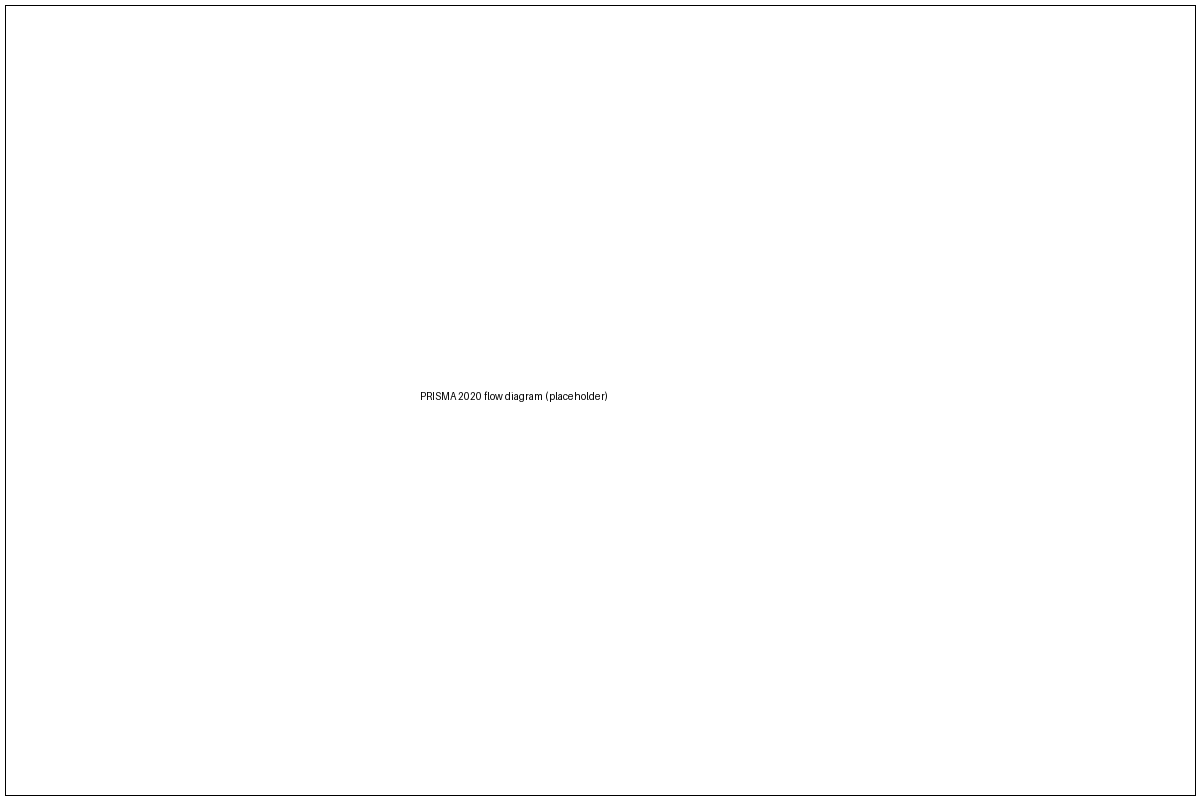
\includegraphics[width=0.92\textwidth]{prisma_2020_RSL.png}
\caption{Diagrama de flujo PRISMA 2020 adaptado a revisiones sistemáticas de ingeniería de software según los lineamientos de Kitchenham y Charters. Reúne en una sola columna la vía de bases de datos y la vía de otros métodos, y distingue los informes no recuperados de los excluidos con motivo.}\label{fig:prisma}
\end{figure}

\subsection{Caracterización del corpus}

El corpus incluido, que se enumera en el Apéndice~\ref{app:corpus}, se distribuye del modo siguiente. Por rol del estudio: 22 propuestas de protección, 9 contramedidas, 3 trabajos que proponen y rompen a la vez y 1 detector; la subárea de contramedidas reúne, por tanto, 13 de los 35 estudios, y la mayoría son ponencias. Por dominio: 22 de clasificación de imágenes, 5 de reconocimiento facial, 4 de aprendizaje multimodal contrastivo y 4 de otros dominios visuales (agrupamiento, seguimiento de vídeo, aprendizaje contrastivo autosupervisado y cámaras de eventos). Por modelo de amenaza máximo evaluado: 22 en A2, 11 en A1 y 2 en A1.5. Por tipo de publicación: 27 ponencias y 8 artículos de revista. Por año: 1 de 2021, 4 de 2023, 12 de 2024, 14 de 2025 y 4 de 2026. Dieciocho de los 35 declaran código o datos disponibles (PC9\,=\,1) y diecisiete registran una dirección de repositorio. Por país de la afiliación de los autores, contando cada país una vez por estudio (12 estudios tienen autores en más de un país): China 26, Singapur 10, Australia 5, Estados Unidos 4, Reino Unido 3 y Alemania 1. Dos rasgos de esta distribución condicionan la lectura de la síntesis y se declaran como amenazas a la validez externa en la Sección~\ref{sec:validez}: la concentración en clasificación de imágenes, que deja las conclusiones sobre reconocimiento facial apoyadas en cinco estudios, y la concentración geográfica de las afiliaciones.

\subsection{Estructura bibliométrica de la literatura}\label{sec:bib-res}

\paragraph{AB1. Producción anual y tendencia.} El corpus temático (141 registros) crece de 8 registros en 2021 a 51 en 2025; los 30 de 2026 corresponden a un año incompleto (la búsqueda se ejecutó en septiembre). La línea facial pasa de dos registros en 2021 a 16 en 2025 (31\,\% del año) y 12 en 2026 (40\,\%). Los 35 estudios incluidos se concentran en 2024 y 2025 (26 de 35), de modo que la comprobación sobre el corpus incluido reproduce el crecimiento descrito. En la tendencia de términos (Figura~\ref{fig:ab1}b), \emph{privacy protection}, \emph{face recognition} y \emph{adversarial examples} están presentes desde 2021; \emph{diffusion models} y \emph{unlearnable examples} aparecen en 2023 y se mantienen o crecen hasta 2026; \emph{facial privacy protection} aparece en 2024; y \emph{poisoning attacks} alcanza su máximo en 2023--2024 (4 y 7 registros) y cae a 2 en 2025 y 1 en 2026.

\begin{figure}[h]
\centering
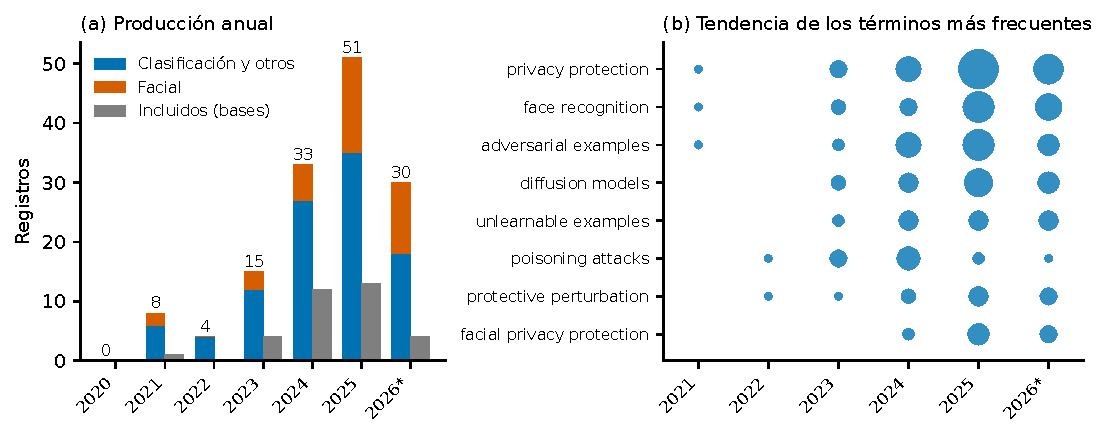
\includegraphics[width=\textwidth]{figuras/AB1_produccion_y_tendencia.pdf}
\caption{(a) Producción anual del corpus temático, con la línea facial en naranja, y de los estudios incluidos procedentes de las bases (gris). (b) Frecuencia anual de los términos más frecuentes; el área de cada círculo es proporcional al número de registros. 2026* es un año incompleto.}\label{fig:ab1}
\end{figure}

\paragraph{AB2. Estructura conceptual.} Entre los 88 registros del corpus temático con palabras clave, la red de co-palabras reúne 82 términos y 179 aristas y se divide en cuatro comunidades de tres o más términos (modularidad 0{,}29) y dos pares aislados (Figura~\ref{fig:ab2}). La primera (C1) agrupa \emph{privacy protection}, \emph{face recognition}, \emph{facial privacy protection} y términos de caja negra y modelo sustituto; la segunda (C2), \emph{diffusion models}, \emph{data protection} y \emph{purification}; la tercera (C3), \emph{unlearnable examples}, \emph{poisoning attacks} y \emph{protective perturbation}; y la cuarta (C4), \emph{adversarial examples}, \emph{contrastive learning} y \emph{copyright protection}. En el mapa temático (Figura~\ref{fig:ab2}b), C1 y C2 se ubican en el cuadrante de centralidad y densidad altas (temas motores), mientras que C3 y C4 quedan en el de centralidad y densidad bajas; C3 contiene el núcleo conceptual del constructo y es la comunidad con menor centralidad. La comprobación sobre los 31 estudios incluidos con palabras clave arroja los mismos términos dominantes: \emph{privacy protection} (13 estudios), \emph{unlearnable examples} (11), \emph{poisoning attacks} (10) y \emph{adversarial examples} (7); nueve de los doce términos más frecuentes del corpus temático están entre los doce del corpus incluido.

\begin{figure}[h]
\centering
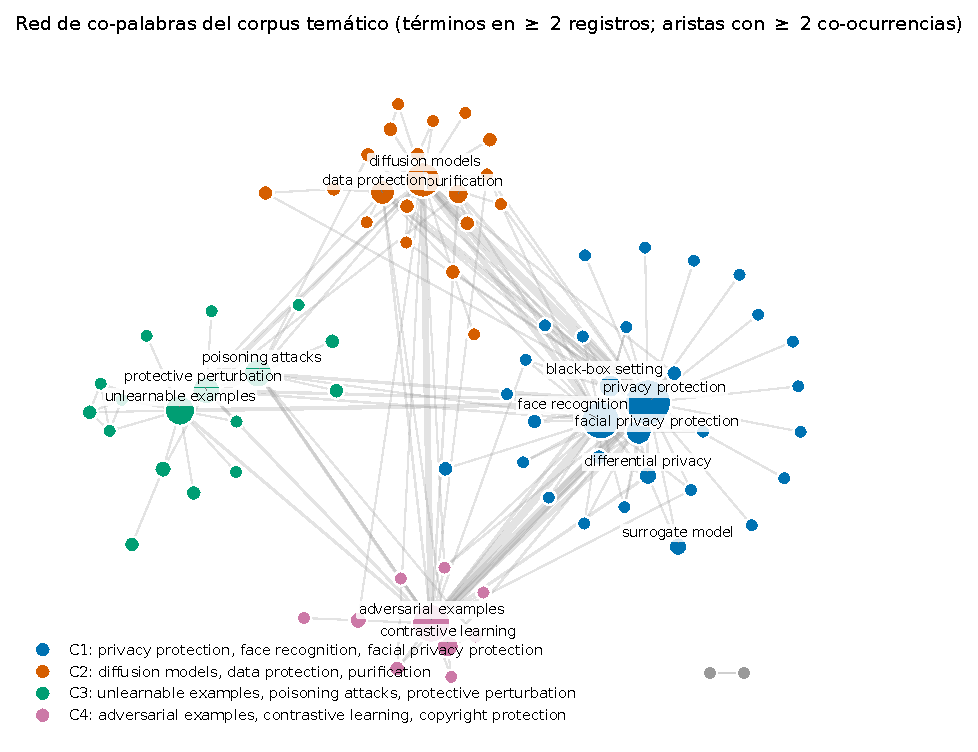
\includegraphics[width=\textwidth]{figuras/AB2_red_copalabras.pdf}
\caption{Red de co-palabras del corpus temático. El tamaño del nodo es proporcional al número de registros y el color indica la comunidad (método de Louvain).}\label{fig:ab2}
\end{figure}

\begin{figure}[h]
\centering
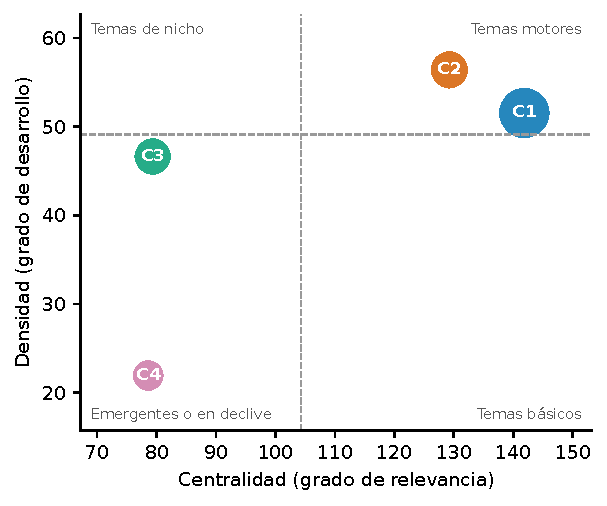
\includegraphics[width=0.62\textwidth]{figuras/AB2_mapa_tematico.pdf}
\caption{Mapa temático de las comunidades de la red de co-palabras: centralidad (relevancia en la red) y densidad (cohesión interna) según Callon et al.; las líneas discontinuas son las medianas.}\label{fig:ab2b}
\end{figure}

\paragraph{AB3. Separación de las líneas de clasificación y facial.} De los 88 registros con palabras clave, 33 pertenecen a la línea facial y 55 a la de clasificación y otros dominios. La proporción media de registros faciales por término es de 0{,}76 en C1, 0{,}44 en C2, 0{,}16 en C3 y 0{,}35 en C4, y la asortatividad ponderada de esa proporción entre términos conectados es de 0{,}48 (media bajo permutación de $-$0{,}07; $p<0{,}001$), de modo que las dos líneas ocupan regiones distintas de la red (Figura~\ref{fig:ab3}). Los términos que las conectan son \emph{privacy protection} (presente en 29 registros faciales y 14 de clasificación), \emph{adversarial examples} (17 y 12) y \emph{diffusion models} (12 y 12), que además tienen la mayor intermediación (0{,}44, 0{,}23 y 0{,}18 para \emph{privacy protection}, \emph{diffusion models} y \emph{unlearnable examples}, respectivamente). Estos resultados son exploratorios: se apoyan en palabras clave disponibles para el 62\,\% del corpus temático y en una red de 82 términos.

\begin{figure}[h]
\centering
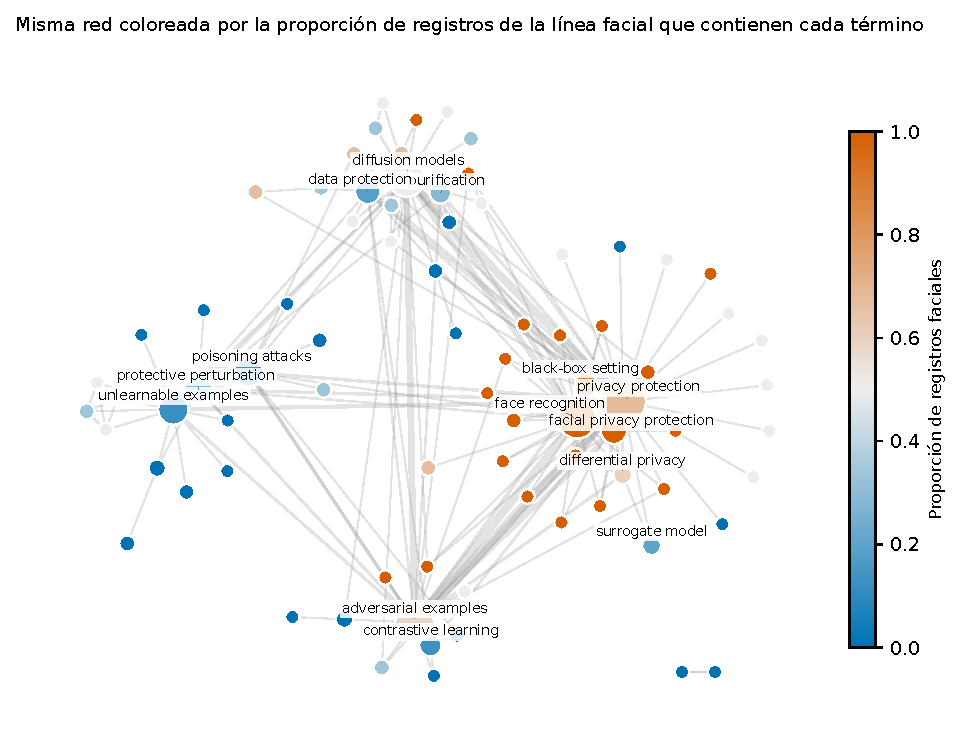
\includegraphics[width=\textwidth]{figuras/AB3_separacion_lineas.pdf}
\caption{Red de co-palabras coloreada por la proporción de registros de la línea facial que contienen cada término (azul: clasificación y otros dominios; naranja: facial).}\label{fig:ab3}
\end{figure}

\subsection{RQ1. Familias de perturbaciones y criterios de clasificación}

De los 35 estudios, 24 proponen una protección; los 11 restantes son contramedidas o detectores y se tratan en RQ2. Las protecciones se clasificaron con cuatro criterios (Tabla~\ref{tab:rq1}). La inserción aditiva en el espacio del píxel es la más frecuente (13 de 24); le siguen la convolucional ---en torno a la familia CUDA \cite{sadasivan2023cuda}---, la basada en el dominio de la frecuencia, la que opera en el espacio de características y la que edita el espacio latente de un generador. Por granularidad predomina la perturbación por muestra (11), seguida de la perturbación por clase (8); dos son universales por clúster y una no reporta la granularidad. La dependencia de un modelo es la norma: nueve protecciones usan un sustituto entrenado, seis un generador entrenado y tres un extractor preentrenado, y solo seis, todas ellas convolucionales o basadas en filtros, no dependen de ningún modelo. El paradigma objetivo es sobre todo la clasificación supervisada (14 de 24); cuatro protecciones apuntan al reconocimiento facial, dos al aprendizaje multimodal y una a cada uno de agrupamiento, seguimiento de vídeo y cámaras de eventos, y una evalúa a la vez el aprendizaje supervisado y el autosupervisado.

Dos observaciones condicionan la comparación. La primera es que ocho protecciones no fijan una cota $L_p$ de perturbación (por ejemplo CUDA, EUN o KBS) y usan en su lugar un parámetro de desenfoque, una pérdida de reconstrucción o un presupuesto de calidad, de modo que no pueden compararse a igual imperceptibilidad (RQ6). La segunda es que solo dos protecciones prevén la reversión autorizada \cite{wang2026reversible,chow2024chameleon}, y que una tercera la afirma sin preverla en el método \cite{wang2025event}.

\begin{table}[h]
\centering
\caption{Clasificación de las 24 protecciones propuestas según los criterios de RQ1. Entre corchetes, los estudios de cada categoría.}\label{tab:rq1}
\footnotesize
\begin{tabularx}{\textwidth}{@{}Y{0.9}Z{0.25}Y{2.2}@{}}
\toprule
Categoría & $n$ & Estudios \\
\midrule
\multicolumn{3}{@{}l}{\textit{Inserción}} \\
Aditiva & 13 & A02, A03, A05, A06, A10, A17, A20, A21, A25, A31, A34, A36, A38 \\
Convolucional & 4 & A04, A12, A15, A16 \\
Espacio de características & 3 & A01, A07, A26 \\
Dominio de la frecuencia & 3 & A11, A18, A37 \\
Espacio latente & 1 & A28 \\
\midrule
\multicolumn{3}{@{}l}{\textit{Granularidad}} \\
Por muestra & 11 & A01, A02, A05, A06, A11, A17, A20, A26, A28, A31, A38 \\
Por clase & 8 & A04, A12, A15, A16, A18, A21, A25, A37 \\
Mixta (muestra y clase) & 2 & A03, A36 \\
Universal por clúster & 2 & A07, A10 \\
No reportada & 1 & A34 \\
\midrule
\multicolumn{3}{@{}l}{\textit{Dependencia de modelo}} \\
Sustituto entrenado & 9 & A06, A07, A20, A21, A25, A28, A31, A34, A36 \\
Generador entrenado & 6 & A02, A03, A05, A10, A17, A37 \\
Sin modelo & 6 & A04, A11, A12, A15, A16, A18 \\
Extractor preentrenado & 3 & A01, A26, A38 \\
\midrule
\multicolumn{3}{@{}l}{\textit{Paradigma objetivo}} \\
Supervisado & 14 & A01, A04, A05, A06, A10, A11, A12, A15, A18, A20, A21, A25, A31, A37 \\
Reconocimiento facial & 4 & A02, A26, A28, A38 \\
Multimodal & 2 & A03, A34 \\
Agrupamiento & 1 & A07 \\
Supervisado y autosupervisado & 1 & A16 \\
Vídeo & 1 & A17 \\
Cámaras de eventos & 1 & A36 \\
\botrule
\end{tabularx}
\end{table}

\subsection{RQ2. Contramedidas documentadas}

Cada estudio evalúa en promedio 3{,}1 tipos de contramedida con cifras (Tabla~\ref{tab:rq2}). Las más extendidas son la transformación o compresión del dato (23 estudios), el entrenamiento robusto (22) y los aumentos de datos (21), seguidas de los recursos iniciales del recolector (18), que incluyen la mezcla con datos limpios, el preentrenamiento y el ajuste fino. La purificación generativa se evalúa en 6 estudios, el cambio de paradigma o de procedimiento en 7 y la detección en 3. Solo ocho estudios evalúan una contramedida diseñada contra un mecanismo concreto: DAT frente a CUDA \cite{sadasivan2023cuda}, COIN \cite{li2025coin}, RSKFF \cite{li2026wavelet,li2025kspace}, ATP \cite{li2025crossmodal}, un módulo de ECLIPSE diseñado contra SEP \cite{wang2024eclipse} y Oriole frente a Fawkes \cite{chen2021oriole}. En tres de ellos la contramedida se aplica a una protección de otro autor sin adaptarla. Dos estudios no evalúan ninguna contramedida de los tipos K1 a K8 \cite{wu2025temporal,ye2024ungeneralizable}. Los resultados de algunas contramedidas solo figuran en figuras (por ejemplo JPEG y aumentos en \cite{zhang2025segue}), lo que introduce incertidumbre de lectura.

\begin{table}[h]
\centering
\caption{Tipos de contramedida evaluados con cifras en los 35 estudios (un estudio puede evaluar varios tipos).}\label{tab:rq2}
\footnotesize
\begin{tabularx}{\textwidth}{@{}cY{1.4}Z{0.25}Y{1.6}@{}}
\toprule
Tipo & Descripción & $n$ & Estudios \\
\midrule
K1 & Transformación o compresión del dato (JPEG, escala de grises, filtros, ISS) & 23 & A04, A06, A08, A09, A10, A11, A12, A14, A15, A16, A18, A19, A20, A23, A25, A26, A28, A30, A32, A33, A35, A37, A38 \\
K2 & Aumento de datos (Mixup, Cutout, CutMix, AutoAugment, UEraser) & 21 & A03, A04, A05, A06, A08, A09, A10, A11, A12, A14, A15, A16, A18, A21, A23, A25, A30, A32, A35, A36, A37 \\
K3 & Entrenamiento robusto (entrenamiento adversarial, suavizado aleatorio, DP-SGD) & 22 & A01, A02, A04, A05, A06, A07, A08, A09, A11, A12, A14, A15, A16, A18, A20, A21, A23, A25, A30, A32, A35, A37 \\
K4 & Purificación generativa (AVATAR, ECLIPSE, JCDP) & 6 & A12, A13, A14, A16, A19, A33 \\
K5 & Cambio de paradigma o de procedimiento (SSL, ensambles, reetiquetado) & 7 & A09, A16, A20, A23, A28, A35, A37 \\
K6 & Recursos iniciales del recolector (preentrenamiento, ajuste fino, datos limpios, mezcla) & 18 & A01, A03, A04, A06, A11, A14, A16, A18, A20, A23, A25, A28, A32, A33, A34, A35, A37, A39 \\
K7 & Detección & 3 & A08, A12, A13 \\
K8 & Contramedida diseñada contra un mecanismo concreto & 8 & A04, A11, A12, A16, A18, A19, A33, A39 \\
\botrule
\end{tabularx}
\end{table}

\subsection{RQ3. Persistencia de la protección y exactitud recuperada}

La Tabla~\ref{tab:persist} del Apéndice~\ref{app:persist} recoge, por estudio, la exactitud sin contramedida, el peor caso para el protector y el residual. Cuatro patrones se repiten.

\textbf{Frente al comparador A0}, las protecciones de clasificación supervisada que reportan CIFAR-10 dejan al adversario entre 10,02\,\% y 28,12\,\% \cite{ma2025t2ue,zhang2026provably}; en ImageNet-100, una protección reversible deja el 6,76\,\% \cite{wang2026reversible} y en Pets una protección por clúster deja el 4,69\,\% \cite{zhang2023clusters}.

\textbf{Frente a las contramedidas que evalúa cada proponente}, el peor caso en CIFAR-10 va de 14,35\,\% (solo aumentos, \cite{ma2025t2ue}) a cerca del 78\,\% \cite{sadasivan2023cuda}, pasando por 19,75\,\% \cite{zhang2023cleanlabel}, 28,73\,\% \cite{li2026wavelet}, 35,07\,\% \cite{chen2025eun}, 54,78\,\% \cite{huang2025imperfect}, 74,5\,\% \cite{zhang2026provably} y 76,96\,\% \cite{liu2024game}. Las evaluaciones más amplias dan los peores casos más altos, y que un estudio solo evalúe aumentos no equivale a que su protección sea resistente.

\textbf{Evaluación por terceros.} Cuando otro estudio diseña la contramedida con conocimiento del mecanismo, el peor caso supera al que declara el proponente: RSKFF y COIN llevan a CUDA a 78,53\,\% y 72,41\,\% \cite{li2025kspace,li2025coin} frente al 51,19\,\% que declara su propio estudio con la configuración por defecto \cite{sadasivan2023cuda}; la purificación por difusión conjunta lleva a UC-CLIP a 47,5\,\% con un limpio de 48,3\,\% \cite{jiang2023false}, frente al 26,11\,\% que reporta su propio estudio \cite{zhang2023clusters}; y la misma contramedida eleva a más del 90\,\% la exactitud sobre protecciones de error minimizado \cite{jiang2023false}.

\textbf{Protección parcial.} Cuando solo una parte del conjunto está protegida, el efecto depende del procedimiento: con entrenamiento estándar, los datos protegidos pueden perjudicar el aprendizaje (--21,48 puntos con la mitad protegida \cite{zhang2026provably}); con entrenamiento adversarial, vuelven a aportar (de +3,3 a +8,3 puntos con el 80\,\% protegido \cite{sadasivan2023cuda,huang2025imperfect,li2025kspace}).

Entre los estudios de contramedida, las recuperaciones reportadas son altas: el 91\,\% de media con purificación por difusión en CIFAR-10 \cite{dolatabadi2024devil}, el 93,1\,\% con LE \cite{jiang2023false}, el 90,84\,\% con ensambles \cite{hapuarachchi2025advancing}, el 83,69\,\% de media con ECLIPSE \cite{wang2024eclipse} y el 86,4\,\% con Noise-JPEG en aprendizaje contrastivo \cite{guo2024jpeg}. Frente a ellas, una protección condicionada a la red autorizada eleva al adversario solo del 26,12\,\% al 35,23\,\% con destilación \cite{ye2024ungeneralizable}. En reconocimiento facial y en aprendizaje multimodal las cifras no son equiparables a las de clasificación: la recuperación media es del 89,0\,\% medida con la mediana del rango \cite{li2025crossmodal}, el ajuste fino de un modelo preentrenado deja la protección en un fallo (Hit@10 de 93,3 frente a 94 con ajuste benigno \cite{liu2024multimodal}) y la exactitud de un adversario con fotos limpias previas pasa de 0,120 a 0,875 \cite{chen2021oriole}.

En 17 de los 35 estudios el residual solo puede calcularse frente a una referencia limpia de entrenamiento estándar (marcada con \textdagger{} en la Tabla~\ref{tab:persist}) o no se reporta, de modo que sobrestima la protección que persiste.%
% NOTA PARA LOS AUTORES: RQ3 usa la referencia limpia propuesta en la decisión A5 (limpia bajo la misma contramedida si existe; si no, estándar con marca). Confirmar.
{}

\subsection{RQ4. Modelos de amenaza}

Según la etiqueta única de máximo nivel evaluado, 22 estudios alcanzan A2, 11 A1 y 2 A1.5. Al distinguir dentro de A2 la contramedida específica del método (A2-e) de la de familia (A2-f), 6 estudios son A2-e y 15 son A2-f (Tabla~\ref{tab:rq4}). La asimetría entre proponentes y contramedidas es el rasgo más claro: de los 25 estudios que proponen una protección, 12 no pasan de un adversario genérico, 2 evalúan uno con preentrenamiento y solo tres diseñan una contramedida contra su propia protección \cite{sadasivan2023cuda,li2025coin,ye2024ungeneralizable}, mientras que los 10 estudios de contramedida o detección construyen adversarios A2-f o A2-e. Los proponentes asumen de forma recurrente que controlan el 100\,\% de los datos, que mantienen secretos (una clave o una máscara) y que disponen de datos limpios etiquetados; ningún estudio evalúa qué ocurre si falla el secreto. Siete estudios \cite{zhu2024detection,jiang2023false,li2025crossmodal,zhang2023cleanlabel,hapuarachchi2025advancing,wang2024eclipse,dolatabadi2024devil} atribuyen al adversario o al titular el uso del conjunto de prueba para elegir hiperparámetros, parar el entrenamiento o fijar umbrales, un recurso poco realista que infla la recuperación reportada y se declara como amenaza a la validez de la síntesis.%
% NOTA PARA LOS AUTORES: la distinción A2-e/A2-f es una variable adicional (decisiones A4 y A6); no modifica la rúbrica de calidad. Confirmar.
{}

\begin{table}[h]
\centering
\caption{Nivel máximo de amenaza evaluado: etiqueta única según la escala A0--A2 y refinamiento de A2 en contramedida específica del método (A2-e) o de la familia (A2-f).}\label{tab:rq4}
\footnotesize
\begin{tabular}{@{}lcccc@{}}
\toprule
Grupo & A1 & A1.5 & A2-e & A2-f \\
\midrule
Proponentes de protección ($n=25$) & 12 & 2 & 3 & 8 \\
Contramedidas y detección ($n=10$) & 0 & 0 & 3 & 7 \\
\midrule
Total ($n=35$) & 12 & 2 & 6 & 15 \\
\botrule
\end{tabular}
\end{table}

\subsection{RQ5. Conjuntos de datos, arquitecturas y modelos objetivo}

La evaluación se concentra en CIFAR-10 (25 de 35 estudios) y en subconjuntos de ImageNet (23), con ResNet-18 como modelo principal o víctima en 26 estudios (Tabla~\ref{tab:rq5}). Once estudios evalúan conjuntos de reconocimiento facial y 11 emplean transformers o modelos CLIP, ya sea como víctima o como sustituto; ocho evalúan paradigmas autosupervisados o contrastivos. La resolución máxima de los conjuntos de clasificación es de 256\,$\times$\,256 píxeles, y ningún estudio evalúa modelos fundacionales ni preentrenamiento a gran escala como contramedida, de modo que la validez externa hacia ese escenario no está cubierta. Cuatro estudios amplían el alcance a vídeo, cámaras de eventos, agrupamiento y plataformas comerciales de entrenamiento.

\begin{table}[h]
\centering
\caption{Conjuntos de datos y arquitecturas más frecuentes (número de estudios que los emplean, de 35).}\label{tab:rq5}
\footnotesize
\begin{tabular}{@{}lc@{\hspace{2em}}lc@{}}
\toprule
Conjunto de datos & $n$ & Arquitectura & $n$ \\
\midrule
CIFAR-10 & 25 & ResNet-18 & 26 \\
Subconjuntos de ImageNet & 23 & VGG & 18 \\
CIFAR-100 & 2 & DenseNet & 17 \\
Conjuntos faciales & 11 & Transformers o CLIP & 11 \\
Tiny ImageNet & 5 &  &  \\
Flickr8k/30k o MS-COCO & 3 &  &  \\
\botrule
\end{tabular}
\end{table}

\subsection{RQ6. Métricas y problemas de comparabilidad}

La métrica dominante es la exactitud de test sobre datos limpios; la complementan métricas de recuperación (Hit@K, mediana del rango), de seguimiento (AO, SR, J\&F), de agrupamiento (ACC, NMI), de detección (HTER, AUC), la tasa de protección y la reidentificación en reconocimiento facial. Solo nueve estudios \cite{zhang2025segue,li2026wavelet,huang2025imperfect,zhang2023cleanlabel,wang2026reversible,fan2025divtrackee,wang2025event,meng2024semantic,chow2024chameleon} reportan una métrica de calidad visual (PSNR, SSIM, LPIPS u otras) y otros dos usan DSSIM solo como presupuesto; el resto no permite comparar las protecciones a igual imperceptibilidad. Cinco estudios reportan repeticiones o semillas \cite{sadasivan2023cuda,liu2024stable,hapuarachchi2025advancing,wang2026reversible,dolatabadi2024devil}. La Tabla~\ref{tab:rq6} resume los problemas de comparabilidad más frecuentes. Su consecuencia es que las exactitudes absolutas no son comparables entre estudios: la exactitud limpia de ResNet-18 en CIFAR-10 varía entre 92,36\,\% y 94,66\,\% según el estudio, y el comparador A0 de CUDA entre 18,48\,\% y 26,49\,\%; conviene usar diferencias dentro de cada estudio.

\begin{table}[h]
\centering
\caption{Problemas de comparabilidad detectados en la extracción y estudios afectados.}\label{tab:rq6}
\footnotesize
\begin{tabularx}{\textwidth}{@{}Y{1.8}Z{0.2}Y{1.3}@{}}
\toprule
Problema & $n$ & Estudios \\
\midrule
La exactitud limpia de referencia no se reporta bajo la misma contramedida (se usa la referencia con entrenamiento estándar) o no se reporta & 17 & A01, A03, A04, A05, A06, A07, A08, A10, A12, A13, A15, A18, A21, A25, A26, A30, A38 \\
Cifras de líneas base reutilizadas de otros estudios sin declararlo & 5 & A11, A15, A18, A21, A25 \\
Valores distintos para una misma configuración entre tablas o entre texto y tablas & 10 & A01, A02, A06, A10, A11, A13, A14, A20, A32, A36 \\
Resultados disponibles solo en figuras & 5 & A01, A02, A10, A21, A38 \\
Presupuesto de perturbación no declarado o inconsistente & 7 & A01, A06, A11, A17, A21, A28, A30 \\
El adversario o el titular usa el conjunto de prueba para decidir & 7 & A08, A14, A19, A21, A23, A33, A35 \\
\botrule
\end{tabularx}
\end{table}

\subsection{RQ7. Variación de la robustez y la reversibilidad según el dominio}

El corpus se reparte en 22 estudios de clasificación, 5 de reconocimiento facial, 4 multimodales y 4 de otros dominios (Tabla~\ref{tab:rq7}). Los protocolos difieren entre dominios en contramedidas, métricas y referencia limpia, de modo que la variación se describe entre estudios y no puede atribuirse al dominio con independencia de esas diferencias. En reconocimiento facial, los cinco estudios usan métricas distintas (exactitud de identificación, tasa de protección frente a Fawkes, tasa de éxito del rastreador, reidentificación) y las contramedidas evaluadas son sobre todo JPEG y filtros, entrenamiento adversarial, la actualización de la galería del rastreador y una contramedida de caja blanca diseñada contra Fawkes; la referencia limpia de la mayoría no se reporta. Cinco estudios de clasificación evalúan además la misma protección en identificación facial de conjunto cerrado \cite{gong2026armor,chen2025eun,liu2024stable,zhang2023cleanlabel,dolatabadi2024devil}, y ninguno evalúa verificación ni conjunto abierto. En los estudios multimodales, la protección falla por componentes propios de la modalidad (el texto) o bajo ajuste fino de un modelo preentrenado \cite{li2025crossmodal,liu2024multimodal}, y en el seguimiento de vídeo la protección conserva entre el 70 y el 77\,\% del rendimiento limpio en segmentación \cite{wu2025temporal}.

Respecto de la reversibilidad, 26 estudios documentan solo una reversión funcional, en la que el adversario recupera la utilidad sin restaurar el dato (entrenamiento adversarial, aumentos, ensambles, ajuste fino, transformaciones); 4 combinan una reversión funcional con una restauración, y 4 se basan en la restauración por purificación. Un estudio no evalúa la reversión por no ser verificable su resultado. Solo dos protecciones prevén la reversibilidad autorizada, y solo una la mide, con una recuperación del 96,6 al 99,6\,\% de la exactitud original \cite{wang2026reversible}. Los estudios que informan una restauración no reportan una medida de fidelidad entre la imagen restaurada y la original en la extracción realizada.%
% NOTA PARA LOS AUTORES: RQ7 sigue la redacción vigente de la pregunta; la reformulación de la condición (ii) del vacío (decisión A8) sigue sujeta a confirmación.
{}

\begin{table}[h]
\centering
\caption{Dominio de evaluación y tipo de reversión por parte del adversario.}\label{tab:rq7}
\footnotesize
\begin{tabular}{@{}lccccc@{}}
\toprule
Dominio & $n$ & Funcional & Mixta & Restaurativa & No evaluada \\
\midrule
Clasificación & 22 & 15 & 3 & 4 & 0 \\
Reconocimiento facial & 5 & 5 & 0 & 0 & 0 \\
Multimodal & 4 & 3 & 1 & 0 & 0 \\
Otros & 4 & 3 & 0 & 0 & 1 \\
\midrule
Total & 35 & 26 & 4 & 4 & 1 \\
\botrule
\end{tabular}
\end{table}

\begin{appendices}

\section{Ecuación PICO: forma literal por plataforma}\label{app:cadenas}

Las cuatro cadenas se ejecutaron el 14 de septiembre de 2026. Cada base se consultó dos veces con la misma cadena: una pasada sin filtros, cuyo recuento de pantalla alimenta la caja de identificación del diagrama de flujo, y una pasada con los filtros que se indican, cuyo archivo exportado es el que se cribó. ScienceDirect no admite la ecuación y ACM Digital Library no permite exportar con el acceso disponible; ambas se declaran conforme al ítem 8 de PRISMA-S.

\subsection{Scopus}
Campo \texttt{TITLE-ABS-KEY}, búsqueda avanzada. Sin filtros: 112 registros.
\begin{quote}\footnotesize\ttfamily\raggedright
TITLE-ABS-KEY ( "unlearnable*" OR \allowbreak "availability poison*" OR \allowbreak "perturbative availability" OR \allowbreak "error-minimizing noise" OR \allowbreak "indiscriminate poisoning" OR \allowbreak "delusive adversar*" OR \allowbreak "unexploitable data" OR \allowbreak "image cloaking" OR \allowbreak "adversarial cloaking" OR \allowbreak "anti-facial recognition" OR \allowbreak "facial privacy protection" OR \allowbreak "protective perturbation*" OR \allowbreak "unauthorized training" OR \allowbreak "unauthorized data usage" OR \allowbreak "unauthorized exploitation" ) AND \allowbreak TITLE-ABS-KEY ( "countermeasure*" OR \allowbreak "defens*" OR \allowbreak "defenc*" OR \allowbreak "defend*" OR \allowbreak "attack*" OR \allowbreak "break*" OR \allowbreak "bypass*" OR \allowbreak "circumvent*" OR \allowbreak "adversarial training" OR \allowbreak "augment*" OR \allowbreak "jpeg" OR \allowbreak "compress*" OR \allowbreak "purif*" OR \allowbreak "ensemble*" OR \allowbreak "distill*" OR \allowbreak "mix*" OR \allowbreak "pre-trained" OR \allowbreak "pre-training" OR \allowbreak "fine-tuning" OR \allowbreak "fine-tuned" ) AND \allowbreak TITLE-ABS-KEY ( "baseline*" OR \allowbreak "clean" OR \allowbreak "existing" OR \allowbreak "previous*" OR \allowbreak "benchmark*" OR \allowbreak "outperform*" OR \allowbreak "original data" OR \allowbreak "original image*" ) AND \allowbreak TITLE-ABS-KEY ( "accurac*" OR \allowbreak "performance*" OR \allowbreak "effective*" OR \allowbreak "success rate*" OR \allowbreak "error" OR \allowbreak "imperceptib*" OR \allowbreak "generaliz*" )
\end{quote}
Filtros de la segunda pasada, añadidos al final de la misma cadena; con ellos el export contiene 109 registros:
\begin{quote}\footnotesize\ttfamily\raggedright
AND ( LIMIT-TO ( DOCTYPE,"cp" ) OR \allowbreak LIMIT-TO ( DOCTYPE,"ar" ) ) AND \allowbreak PUBYEAR > 2019 AND \allowbreak PUBYEAR < 2027
\end{quote}
Advertencia de plataforma: Scopus no expande el comodín situado después de un guion, de modo que \texttt{"pre-train*"} y \texttt{"fine-tun*"} no devuelven resultados. Por eso la cadena escribe las cuatro formas explícitas.

\subsection{Web of Science}
Búsqueda avanzada, campo \texttt{TS=} (Topic). Sin filtros: 28 registros. Filtros de la segunda pasada: \emph{Publication Years} 2020--2026 y \emph{Document Types} \emph{Article} y \emph{Proceedings Paper}; no se refinó por idioma. Los filtros no eliminan ningún registro.
\begin{quote}\footnotesize\ttfamily\raggedright
TS=("unlearnable*" OR \allowbreak "availability poison*" OR \allowbreak "perturbative availability" OR \allowbreak "error-minimizing noise" OR \allowbreak "indiscriminate poisoning" OR \allowbreak "delusive adversar*" OR \allowbreak "unexploitable data" OR \allowbreak "image cloaking" OR \allowbreak "adversarial cloaking" OR \allowbreak "anti-facial recognition" OR \allowbreak "facial privacy protection" OR \allowbreak "protective perturbation*" OR \allowbreak "unauthorized training" OR \allowbreak "unauthorized data usage" OR \allowbreak "unauthorized exploitation") AND \allowbreak TS=("countermeasure*" OR \allowbreak "defens*" OR \allowbreak "defenc*" OR \allowbreak "defend*" OR \allowbreak "attack*" OR \allowbreak "break*" OR \allowbreak "bypass*" OR \allowbreak "circumvent*" OR \allowbreak "adversarial training" OR \allowbreak "augment*" OR \allowbreak "jpeg" OR \allowbreak "compress*" OR \allowbreak "purif*" OR \allowbreak "ensemble*" OR \allowbreak "distill*" OR \allowbreak "mix*" OR \allowbreak "pre-trained" OR \allowbreak "pre-training" OR \allowbreak "fine-tuning" OR \allowbreak "fine-tuned") AND \allowbreak TS=("baseline*" OR \allowbreak "clean" OR \allowbreak "existing" OR \allowbreak "previous*" OR \allowbreak "benchmark*" OR \allowbreak "outperform*" OR \allowbreak "original data" OR \allowbreak "original image*") AND \allowbreak TS=("accurac*" OR \allowbreak "performance*" OR \allowbreak "effective*" OR \allowbreak "success rate*" OR \allowbreak "error" OR \allowbreak "imperceptib*" OR \allowbreak "generaliz*")
\end{quote}
\subsection{IEEE Xplore}
\emph{Advanced Search} $\rightarrow$ \emph{Command Search}. Sin filtros: 45 registros. Filtros de la segunda pasada: \emph{Year} 2020--2026 y \emph{Content Type} \emph{Conferences} y \emph{Journals}; no se refinó por idioma. Los filtros no eliminan ningún registro.
\begin{quote}\footnotesize\ttfamily\raggedright
(("All Metadata":"unlearnable*") OR \allowbreak ("All Metadata":"availability poisoning") OR \allowbreak ("All Metadata":"perturbative availability") OR \allowbreak ("All Metadata":"error-minimizing noise") OR \allowbreak ("All Metadata":"indiscriminate poisoning") OR \allowbreak ("All Metadata":"delusive adversarial") OR \allowbreak ("All Metadata":"unexploitable data") OR \allowbreak ("All Metadata":"image cloaking") OR \allowbreak ("All Metadata":"adversarial cloaking") OR \allowbreak ("All Metadata":"anti-facial recognition") OR \allowbreak ("All Metadata":"facial privacy protection") OR \allowbreak ("All Metadata":"protective perturbation") OR \allowbreak ("All Metadata":"unauthorized training") OR \allowbreak ("All Metadata":"unauthorized data usage") OR \allowbreak ("All Metadata":"unauthorized exploitation")) AND \allowbreak (("All Metadata":"defens*") OR \allowbreak ("All Metadata":"attack*") OR \allowbreak ("All Metadata":"augment*") OR \allowbreak ("All Metadata":"purif*") OR \allowbreak ("All Metadata":"countermeasure") OR \allowbreak ("All Metadata":"countermeasures") OR \allowbreak ("All Metadata":"defence") OR \allowbreak ("All Metadata":"defend") OR \allowbreak ("All Metadata":"break") OR \allowbreak ("All Metadata":"breaking") OR \allowbreak ("All Metadata":"adversarial training") OR \allowbreak ("All Metadata":"compression") OR \allowbreak ("All Metadata":"pre-trained") OR \allowbreak ("All Metadata":"pre-training") OR \allowbreak ("All Metadata":"fine-tuning") OR \allowbreak ("All Metadata":"mixup") OR \allowbreak ("All Metadata":"mixed") OR \allowbreak ("All Metadata":"ensemble") OR \allowbreak ("All Metadata":"ensembles") OR \allowbreak ("All Metadata":"jpeg") OR \allowbreak ("All Metadata":"distillation")) AND \allowbreak (("All Metadata":"baseline") OR \allowbreak ("All Metadata":"baselines") OR \allowbreak ("All Metadata":"clean") OR \allowbreak ("All Metadata":"existing") OR \allowbreak ("All Metadata":"previous") OR \allowbreak ("All Metadata":"benchmark") OR \allowbreak ("All Metadata":"outperform") OR \allowbreak ("All Metadata":"outperforms") OR \allowbreak ("All Metadata":"original data") OR \allowbreak ("All Metadata":"original images")) AND \allowbreak (("All Metadata":"accurac*") OR \allowbreak ("All Metadata":"effective*") OR \allowbreak ("All Metadata":"generaliz*") OR \allowbreak ("All Metadata":"imperceptib*") OR \allowbreak ("All Metadata":"performance") OR \allowbreak ("All Metadata":"error") OR \allowbreak ("All Metadata":"success rate"))
\end{quote}
Advertencias de plataforma: el \emph{Command Search} admite un máximo de diez comodines por consulta, de los cuales la cadena usa nueve y escribe el resto de plurales y variantes de forma explícita; y el campo \emph{All Metadata} busca en más campos que título, resumen y palabras clave, por lo que IEEE Xplore recupera registros que Scopus no devuelve con el mismo constructo.

\subsection{SpringerLink}
Buscador general de la plataforma. Sin filtros: 533 registros. Filtros de la segunda pasada: \emph{Content Type} \emph{Article} y \emph{Conference Paper} y \emph{Publication Year} 2020--2026; con ellos el export contiene 232 registros.
\begin{quote}\footnotesize\ttfamily\raggedright
("adversarial cloaking" OR \allowbreak "anti-facial recognition" OR \allowbreak "availability poison" OR \allowbreak "availability poisoning" OR \allowbreak "delusive adversarial" OR \allowbreak "error-minimizing noise" OR \allowbreak "facial privacy protection" OR \allowbreak "image cloaking" OR \allowbreak "indiscriminate poisoning" OR \allowbreak "perturbative availability" OR \allowbreak "protective perturbation" OR \allowbreak "protective perturbations" OR \allowbreak "unauthorized data usage" OR \allowbreak "unauthorized exploitation" OR \allowbreak "unauthorized training" OR \allowbreak "unexploitable data" OR \allowbreak "unlearnable") AND \allowbreak ("adversarial training" OR \allowbreak "attack" OR \allowbreak "attacks" OR \allowbreak "augmentation" OR \allowbreak "break" OR \allowbreak "breaking" OR \allowbreak "bypass" OR \allowbreak "bypassing" OR \allowbreak "circumvent" OR \allowbreak "compression" OR \allowbreak "countermeasure" OR \allowbreak "countermeasures" OR \allowbreak "defence" OR \allowbreak "defences" OR \allowbreak "defend" OR \allowbreak "defending" OR \allowbreak "defense" OR \allowbreak "defenses" OR \allowbreak "defensive" OR \allowbreak "distillation" OR \allowbreak "ensemble" OR \allowbreak "fine-tuned" OR \allowbreak "fine-tuning" OR \allowbreak "jpeg" OR \allowbreak "mixed" OR \allowbreak "mixup" OR \allowbreak "pre-trained" OR \allowbreak "pre-training" OR \allowbreak "purification") AND \allowbreak ("baseline" OR \allowbreak "baselines" OR \allowbreak "benchmark" OR \allowbreak "clean" OR \allowbreak "existing" OR \allowbreak "original data" OR \allowbreak "original images" OR \allowbreak "outperform" OR \allowbreak "outperforms" OR \allowbreak "previous") AND \allowbreak ("accuracy" OR \allowbreak "effective" OR \allowbreak "effectiveness" OR \allowbreak "error" OR \allowbreak "generalization" OR \allowbreak "imperceptible" OR \allowbreak "performance" OR \allowbreak "success rate")
\end{quote}
Advertencias de plataforma: el export no incluye resumen ni palabras clave y concatena los autores sin separador, de modo que 221 registros se cribaron por título; y la plataforma no evalúa la conjunción booleana de forma estricta, por lo que su recuento no es comparable con el de las demás bases. Ambas circunstancias se declaran como incidencia conforme a PRISMA-S.


\section{Persistencia reportada por estudio}\label{app:persist}

\begin{longtable}{@{}L{0.95cm}L{2.7cm}L{2.2cm}L{3.5cm}L{2.2cm}@{}}
\caption{Persistencia reportada por estudio. A0: exactitud (o métrica equivalente) sin contramedida; peor caso: mayor recuperación del adversario o mejor contramedida; residual: referencia limpia menos exactitud tras la contramedida, en puntos porcentuales. \textdagger{}: la referencia limpia corresponde al entrenamiento estándar y no al mismo procedimiento que la contramedida; [I]: valor calculado a partir de las cifras del estudio.}\label{tab:persist}\\
\toprule
ID & Referencia limpia & A0 & Peor caso o mejor contramedida & Residual \\
\midrule
\endfirsthead
\toprule
ID & Referencia limpia & A0 & Peor caso o mejor contramedida & Residual \\
\midrule
\endhead
\botrule
\endfoot
A01 & ERM\textdagger{} 95,04 (ResNet-18; la T1) & 28,12 (CIFAR-10) & 74,5 (AT PGD, radio no declarado) & 20,54\textdagger{} [I] \\
A02 & Limpio con AT: 65,50 & 10,50 (WebFace10) & 34,00 (AT 4/255, $\rho$\_d = 0); 16,50 con $\rho$\_d = 4 & 31,50 [I] \\
A03 & ERM\textdagger{} 90,34 (con MixUp: 86,17) & 10,02 (CIFAR-10, por clase) & 14,35 (aumentos, T6); 11,44 con MixUp & 75,99\textdagger{} [I] \\
A04 & ERM\textdagger{} 94,66 (limpio con AT 4/255 sí reportado) & 18,48 (ERM, CIFAR-10) & $\approx$ 78 (DAT, p\_b = 0,1); 51,19 por defecto; 78,53 de terceros (RSKFF, A18) & $\approx$ 16,7\textdagger{} [I] \\
A05 & ERM\textdagger{} 92,36 & 13,25 & 76,96 (AT 4/255) & 15,40\textdagger{} [I] \\
A06 & Limpio bajo cada contramedida (sin \textdagger{}) & 12,85 (ResNet-18) & 34,38 (AT Propagate $\rho$ = 2); 28,84 con DeepAA & 56,78 (AT $\rho$ = 2); 65,65 (DeepAA) [I] \\
A07 & ERM\textdagger{} 92,38 (VaDE/MNIST) & 11,25 (VaDE/MNIST) & 11,25 (defensa de Yang et al.; no verificable) & 81,13\textdagger{} [I] con reserva \\
A08 & NR (sin limpio sin veneno) & 10,09 (Err-min(S), CIFAR-10) & 88,01 (AN+SDA); 84,00 (AT) & NR; recuperado +77,92 pp [I] \\
A09 & Limpio SL ImageNet-100: 77,66 & 21,41 (SL, media ImageNet-100) & 55,37 (VESPR); 45,20 en CUDA & 22,29 [I]; recuperado +33,96 pp \\
A10 & ERM\textdagger{} 62,31 (Pets); SimCLR limpio 48,3 & 4,69 (Pets, UC-CLIP) & 26,11 (SimCLR); 18,59 (suavizado); 47,5 con LE/JCDP de terceros (A14) & 0,8 (LE/JCDP con SimCLR, A14) [I] \\
A11 & Limpio con AT: 89,51 (ERM 94,66) & 11,36 (ERM) & 28,73 (RSKFF aplicado bajo AT 4/255) & 60,78 [I] \\
A12 & NR (sin limpio ni presupuesto de AT) & 24,92 (CUDA, media CIFAR-10) & 72,41 (COIN); 47,04 (mejor defensa previa, AT) & NR; recuperado +47,49 pp [I] \\
A13 & NR (ninguna referencia limpia) & NA (detección) & 90,61 (exactitud tras IF + DiffPure sobre lo detectado) & NR \\
A14 & Limpio reportado: 95,3 (T3: 94,7 vanilla) & 21,2 (EMN, CIFAR-10) & 93,1 (LE/JCDP); REMN 92,2 & 2,2 [I] \\
A15 & ERM\textdagger{} 94,66 (sin limpio bajo AT 8/255 ni L2) & 14,15 & 35,07 (UEraser-Max); 19,11 con AT 4/255 & 59,59\textdagger{} [I] \\
A16 & SL limpio 93,86 & 10,39 (SL) & 54,78 (AVATAR); 43,24 (SSL); CUDA 71,90 con COIN & 39,08\textdagger{} [I] \\
A17 & Limpio HIPTrack 77,4 (SeqTrack 74,7) & AO 2,1 (SeqTrack-256) & AO 43,2 (HIPTrack, base congelada; K6 (parcial)) & 34,2 [I] \\
A18 & ERM\textdagger{} 94,66 & 13,53 & 42,53 (RSKFF); 20,97 con AT & 52,13\textdagger{} [I] \\
A19 & Limpio Flickr8K: 27,4 & 4,3 (MEM-3, Flickr8K R@10 I$\rightarrow$T) & 27,5 (CMCR) & $-$0,1 [I] \\
A20 & Limpio con AT 4/255: 89,51 & 13,0 & 77,85 (DenseNet-121, AT 4/255); 57,48 (early stopping); 89,30 si $\rho$\_a se subestima & 57,59 (ResNet-18, AT 4/255) [I] \\
A21 & ERM\textdagger{} 95,43 (RegNet) & 10,54 (úsese con reserva) & 19,75 (AT, sin parámetros declarados) & 75,68\textdagger{} [I] \\
A23 & $\approx$ 95 (valor citado) & 24,34 (EMin, CIFAR-10) & 90,84 (ensemble bagging) & $\approx$ 4,16\textdagger{} [I] \\
A25 & ERM\textdagger{} 72,78 (ImageNet-100, $\varepsilon$ = 4) & 6,76 (ImageNet-100); 11,79 (CIFAR-10) & 63,53 (JPEG QF75); 39,12 con JPEG diferenciable & 9,25\textdagger{} [I] \\
A26 & NR (reidentificación limpia no reportada) & 3,8 (reidentificación) & 6,9 (JPEG-50) & NR \\
A28 & Sin protección con DynTracker: 99,62 (T3) & TSR 28,47--44,25 (A0 estático, T1) & TSR 98,04 (Clip2Protect + DynTracker); DivTrackee 22,16--52,37 & 1,58 (Clip2Protect) [I] \\
A30 & ERM\textdagger{} 91,8 (SimCLR, CIFAR-10) & 44,9 (CPS) & 86,4 (Noise-JPEG); 87,4 en BYOL & 5,4\textdagger{} (CPS); 3,9--8,5\textdagger{} en 12 celdas [I] \\
A31 & Limpio con destilación: 95,41 & 26,12 (hacker ResNet-18) & 35,23 (destilación desde la red autorizada) & 60,18 [I] \\
A32 & Limpio propio de A$^{3}$: 83,60 (T2) & 65,31 (CoCoOp, EM) & 82,27 (A$^{3}$, T2); resumen: 82,43 & 1,33 [I] \\
A33 & Referencia limpia de la misma red ($\approx$ 90,43) & 27,17 (media, ResNet18) & 83,69 (ECLIPSE, media de 9 columnas); 83,82 con 8 venenos & 6,74 [I] \\
A34 & Hit@10 limpio: 46,5 (Flickr30k) & 3,8 (MEM-3, Hit@10 I$\rightarrow$T) & 93,3 (fine-tuning ViT-B/32; benigno 94) $\cdot$ fallo de protección & 0,7 [I] \\
A35 & Limpio con AVATAR: 90,16 (T VI) & 24,85 (EMN) & 90,95 (AVATAR, EMN); 88,49 (REMN) & $-$0,79 (EMN); +1,67 (REMN) [I] \\
A36 & Dc = 78,12 (RN18, N-Caltech101; varía 78,12--78,52) & 0,52 (sample-wise, RN18) & 13,04 (aumentos; E5 = ablación sample-wise) & 65,08 [I] \\
A37 & Limpio por procedimiento (ERM 94,59) & 10,08 (DH class-wise, vanilla) & 83,98 (JPEG10); 82,21 (AT L$\infty$) & 1,24 (JPEG10); 1,98 (AT) [I] \\
A38 & 100 \% sin protección; limpio con filtro NR \textdagger{} & Exactitud FR 3,75 (PSR 96,25) & PSR $\approx$ 81 (filtro gaussiano); PSR 72,56 con el equipo menos diverso & NR \\
A39 & Sin protección: 0,976 (n = 1 usuario) & 0,120 (solo Fawkes) & 0,875 (Oriole, $\rho$ = 0,008, m = 20) & 0,101 [I] \\
\end{longtable}

\section{Estudios incluidos}\label{app:corpus}

Los 35 estudios incluidos en la síntesis, tras el cribado, la elegibilidad a texto completo, la rúbrica de calidad y la selección final. Rol: P propuesta de protección, C contramedida, P$+$C ambas, D detección. Amenaza: etiqueta máxima evaluada en el estudio, según la escala de la Sección~\ref{sec:antecedentes}. QA: puntuación total sobre 9. Los identificadores no se renumeran tras la selección final.

\footnotesize\setlength{\tabcolsep}{3pt}
\begin{longtable}{@{}cL{5.35cm}C{0.8cm}C{0.9cm}C{1.8cm}C{1.35cm}C{0.6cm}@{}}
\caption{Corpus incluido en la síntesis.}\label{tab:corpus}\\
\toprule
ID & Estudio & Año & Rol & Dominio & Amenaza & QA \\
\midrule
\endfirsthead
\toprule
ID & Estudio & Año & Rol & Dominio & Amenaza & QA \\
\midrule
\endhead
\botrule
\endfoot
A01 & Towards Provably Unlearnable Examples via Bayes Error Optimisation~\cite{zhang2026provably} & 2026 & P & Clasificación & A1 & 7{,}0 \\
A02 & Segue: Side-information Guided Generative Unlearnable Examples for Facial Privacy Protection in Real World~\cite{zhang2025segue} & 2025 & P & Facial & A1 & 6{,}5 \\
A03 & T2UE: Generating Unlearnable Examples from Text Descriptions~\cite{ma2025t2ue} & 2025 & P & Multimodal & A1 & 7{,}5 \\
A04 & CUDA: Convolution-Based Unlearnable Datasets~\cite{sadasivan2023cuda} & 2023 & P & Clasificación & A2 & 9{,}0 \\
A05 & Game-Theoretic Unlearnable Example Generator~\cite{liu2024game} & 2024 & P & Clasificación & A1 & 8{,}5 \\
A06 & Armor: Shielding Unlearnable Examples Against Data Augmentation~\cite{gong2026armor} & 2026 & P & Clasificación & A1 & 7{,}5 \\
A07 & Novel poisoning attacks for clustering methods via robust feature generation~\cite{zhang2024clustering} & 2024 & P & Otro & A1 & 6{,}5 \\
A08 & Detection and Defense of Unlearnable Examples~\cite{zhu2024detection} & 2024 & C & Clasificación & A2 & 8{,}5 \\
A09 & Exploiting Supervised Poison Vulnerability to Strengthen Self-supervised Defense~\cite{styborski2025exploiting} & 2025 & C & Clasificación & A2 & 8{,}0 \\
A10 & Unlearnable Clusters: Towards Label-Agnostic Unlearnable Examples~\cite{zhang2023clusters} & 2023 & P & Clasificación & A1 & 7{,}5 \\
A11 & Wavelet Domain Steganography for Robust Unlearnable Data~\cite{li2026wavelet} & 2026 & P & Clasificación & A2 & 7{,}5 \\
A12 & Detecting and Corrupting Convolution-based Unlearnable Examples~\cite{li2025coin} & 2025 & P$+$C & Clasificación & A2 & 8{,}0 \\
A13 & Unlearnable Examples Detection via Iterative Filtering~\cite{yu2024iterative} & 2024 & D & Clasificación & A2 & 6{,}0 \\
A14 & Unlearnable Examples Give a False Sense of Security: Piercing through Unexploitable Data with Learnable Examples~\cite{jiang2023false} & 2023 & C & Clasificación & A2 & 8{,}0 \\
A15 & EUN: Enhanced unlearnable examples generation approach for privacy protection~\cite{chen2025eun} & 2025 & P & Clasificación & A2 & 6{,}5 \\
A16 & Leveraging Imperfect Restoration for Data Availability Attack~\cite{huang2025imperfect} & 2025 & P & Clasificación & A2 & 8{,}5 \\
A17 & Temporal Unlearnable Examples: Preventing Personal Video Data from Unauthorized Exploitation by Object Tracking~\cite{wu2025temporal} & 2025 & P & Otro & A1.5 & 6{,}0 \\
A18 & K-Space Bispectrum Steganography for Robust Unlearnable Data~\cite{li2025kspace} & 2025 & P & Clasificación & A2 & 6{,}5 \\
A19 & Cross-Modal Collaborative Recovery: Breaking Multimodal Unlearnable Examples Protection~\cite{li2025crossmodal} & 2025 & C & Multimodal & A2 & 6{,}5 \\
A20 & Stable Unlearnable Example: Enhancing the Robustness of Unlearnable Examples via Stable Error-Minimizing Noise~\cite{liu2024stable} & 2024 & P & Clasificación & A1 & 8{,}0 \\
A21 & Clean-label poisoning attack with perturbation causing dominant features~\cite{zhang2023cleanlabel} & 2023 & P & Clasificación & A1 & 6{,}0 \\
A23 & Advancing ensemble learning against unlearnable data~\cite{hapuarachchi2025advancing} & 2025 & C & Clasificación & A2 & 8{,}0 \\
A25 & Reversible Unlearnable Examples: Toward the Copyright Protection in Deep Learning Era~\cite{wang2026reversible} & 2026 & P & Clasificación & A2 & 8{,}5 \\
A26 & Protecting Personal Privacy Against Unauthorized Facial Recognition Models via Image Cloaking~\cite{guo2025pyrfawkes} & 2025 & P & Facial & A1 & 6{,}5 \\
A28 & DivTrackee versus DynTracker: Promoting Diversity in Anti-Facial Recognition against Dynamic FR Strategy~\cite{fan2025divtrackee} & 2025 & P$+$C & Facial & A2 & 9{,}0 \\
A30 & Defense Contrastive Poisoning: An Application of JPEG to Self-Supervised Contrastive Learning Indiscriminate Poisoning Attacks~\cite{guo2024jpeg} & 2024 & C & Otro & A2 & 7{,}0 \\
A31 & Ungeneralizable Examples~\cite{ye2024ungeneralizable} & 2024 & P & Clasificación & A2 & 8{,}0 \\
A32 & A3: Few-shot Prompt Learning of Unlearnable Examples with Cross-Modal Adversarial Feature Alignment~\cite{wang2025a3} & 2025 & P$+$C & Multimodal & A2 & 7{,}0 \\
A33 & ECLIPSE: Expunging Clean-Label Indiscriminate Poisons via Sparse Diffusion Purification~\cite{wang2024eclipse} & 2024 & C & Clasificación & A2 & 9{,}0 \\
A34 & Multimodal Unlearnable Examples: Protecting Data against Multimodal Contrastive Learning~\cite{liu2024multimodal} & 2024 & P & Multimodal & A1.5 & 8{,}0 \\
A35 & The Devil's Advocate: Shattering the Illusion of Unexploitable Data using Diffusion Models~\cite{dolatabadi2024devil} & 2024 & C & Clasificación & A2 & 8{,}5 \\
A36 & Asynchronous Event Error-Minimizing Noise for Safeguarding Event Dataset~\cite{wang2025event} & 2025 & P & Otro & A1 & 8{,}5 \\
A37 & Semantic Deep Hiding for Robust Unlearnable Examples~\cite{meng2024semantic} & 2024 & P & Clasificación & A2 & 7{,}5 \\
A38 & Personalized Privacy Protection Mask Against Unauthorized Facial Recognition~\cite{chow2024chameleon} & 2024 & P & Facial & A2 & 8{,}0 \\
A39 & Oriole: Thwarting Privacy Against Trustworthy Deep Learning Models~\cite{chen2021oriole} & 2021 & C & Facial & A2 & 8{,}0 \\
\end{longtable}

\end{appendices}

\bibliography{sn-bibliography}

\end{document}
